%% Manuscript draft v0.3 (2026-10-28), compact version (<= 30 pages). Full v0.2 is in ../archive/manuscript_v0.2_full.
%% Elsevier elsarticle, author-year (Biosystems Engineering style). Supporting tables/figures are in supplementary.tex.
%% Red [TBD: ...] marks results that are still running (closed-loop evaluation) or text to verify.
%% Numbers outside [TBD] come from paper/results/*.json (scripts in paper/experiments/).
\documentclass[preprint,12pt,authoryear]{elsarticle}

\usepackage{lmodern}
\usepackage{amsmath,amssymb}
\usepackage{graphicx}
\usepackage{booktabs}
\usepackage{array}
\usepackage{multirow}
\usepackage{xcolor}
\usepackage{algorithm}
\usepackage{algpseudocode}
\usepackage{siunitx}
\usepackage[colorlinks=true,linkcolor=blue!50!black,citecolor=blue!50!black,urlcolor=blue!50!black]{hyperref}
\usepackage{lineno}
\usepackage{adjustbox}
\usepackage[font=small,labelfont=bf,skip=4pt]{caption}
\usepackage{etoolbox}
\makeatletter\patchcmd{\pprintMaketitle}{\vskip36pt}{\vskip20pt}{}{}\makeatother
\setlength{\emergencystretch}{2em}
\linenumbers

\graphicspath{{../figures/}}
\newcommand{\tbd}[1]{\textcolor{red}{[TBD: #1]}}
\newcommand{\pekm}{PEKM}
\newcommand{\fdm}{SAM-FDM}
\newcommand{\bench}{HarvestMem-Sim}
\sisetup{detect-all}

\renewcommand{\topfraction}{0.9}
\renewcommand{\bottomfraction}{0.8}
\renewcommand{\textfraction}{0.07}
\renewcommand{\floatpagefraction}{0.85}
\setcounter{topnumber}{3}
\setcounter{bottomnumber}{2}
\setcounter{totalnumber}{4}
\setlength{\textfloatsep}{10pt plus 2pt minus 2pt}
\setlength{\floatsep}{8pt plus 2pt minus 2pt}

\journal{Biosystems Engineering}

\begin{document}

\begin{frontmatter}

\title{HarvestMem: event-centric memory for vision--\hspace{0pt}language--\hspace{0pt}action harvesting robots under foliage occlusion}

\author[a]{\tbd{Author 1}}
\author[a]{\tbd{Author 2}}
\author[a]{\tbd{Corresponding author}\corref{cor1}}
\cortext[cor1]{Corresponding author. E-mail: \tbd{email}}
\address[a]{\tbd{Affiliation, city, postcode, country}}

\begin{abstract}
Selective harvesting robots must act on information they can no longer see: wind-blown foliage hides ripe fruits, and quotas depend on picks made outside the camera view. Vision--language--action (VLA) policies, however, remember a fixed number of past frames sampled uniformly in time, and we show that their coverage of completed picks decays inversely with operating time. We propose HarvestMem, an event-centric memory framework that indexes memory by physical interaction events. Its spatial memory, built by a SAM-based fruit distance module (SAM-FDM), anchors every fruit in 3D while it is visible. Its episodic memory, Picking-Event Keyframe Memory (PEKM), detects picks from the end-effector-to-fruit distance and reserves memory slots for their contact and detachment keyframes, without extra parameters or inference cost. On HarvestMem-Sim, a new benchmark with a 7-DoF arm, foliage occlusion and quota counting, PEKM retained 99.6\% of completed picks versus 57.0\% for uniform memory, and with 8 frames outperformed uniform memory with 16. From RGB-D images and proprioception alone, SAM-FDM localized fruits within 0.48~cm and reproduced the ground-truth picking events exactly. Anchored before occlusion, it kept all 138 leaf-hidden ripe fruits (anchor recall 99.8\%); anchored after occlusion, it kept none (78.3\%), and no occluded episode was counted correctly. \tbd{one sentence on closed-loop success}
\end{abstract}

%% Highlights are submitted as a separate file (highlights.tex), as required by Elsevier.

\begin{keyword}
Selective harvesting \sep Vision--language--action model \sep Temporal memory \sep Keyframe selection \sep Foliage occlusion \sep Segment Anything Model
\end{keyword}

\end{frontmatter}

\section*{Nomenclature}
\begin{tabular}{lp{10.8cm}}
$B$ & memory budget (number of past frames kept), here $B=16$\\
$c_U(t)$ & coverage of a completed pick by uniform memory at decision time $t$\\
$S_e$, $W$ & key set of event $e$ (frames within $\pm W$ of its contact and release keyframes), $W=3$\\
$d_t$, $\hat d_t$ & ground-truth and perceived distance from the TCP to the nearest pickable fruit at frame $t$ (m)\\
$\mathcal{P}_t$ & set of pickable fruits still attached at frame $t$\\
$k$ & maximum number of event keyframes reserved in the memory\\
$r$, $\mathrm{tol}$ & event radius and contact tolerance (m)\\
$t^{\mathrm{c}}$, $t^{\mathrm{r}}$ & contact and release keyframes of an event\\
$\mathcal{M}_t$ & set of past frames in the memory at decision time $t$\\
$\alpha$, $\tau_d$ & mixing weight and distance scale of PEKM-S\\
$\sigma$, $\tau$ & stationary standard deviation (rad) and correlation time (steps) of the DART-H noise\\
DART & disturbances for augmenting robot trajectories \citep{laskey2017dart}\\
EV & event memory; EVU, EVR, EVA: its uniform, random-replacement and anti-event controls\\
FDM & fruit distance module\\
PEKM & picking-event keyframe memory\\
TCP & tool centre point\\
VLA & vision--language--action (policy)\\
\end{tabular}

\section{Introduction}
\label{sec:intro}

Harvesting is among the most labour-intensive operations in fruit production, and the shrinking seasonal workforce has made robotic selective harvesting a long-standing goal of agricultural engineering \citep{bac2014harvesting,kootstra2021selective,zhou2022intelligent}. Systems for sweet pepper \citep{arad2020sweetpepper}, kiwifruit \citep{williams2019kiwifruit} and apple \citep{silwal2017apple} are pipelines of detection, localization, planning and grasping modules engineered for one crop, one decision rule and one scene layout. Vision--language--action (VLA) policies offer a different paradigm: a single network pretrained on web-scale vision--language data and large robot datasets maps images, proprioception and a natural-language instruction directly to actions \citep{brohan2023rt2,kim2024openvla,black2024pi0,pi05_2025}, so that \emph{which} fruits to pick, \emph{how many} and \emph{where} to put them become an instruction rather than an engineering effort.

\paragraph{Harvesting is a memory problem} A harvesting robot rarely has in view the information it needs for its next decision. Wind or the manipulator moves leaves over ripe fruits that were visible moments earlier \citep{hemming2014detectability}; grading, sampling and thinning require a given number of fruits; and the collection bin is usually outside the camera's view, so earlier picks cannot be re-observed. Forgetting has a direct agronomic cost: a forgotten ripe fruit is lost yield left to over-mature on the plant, a forgotten pick leads to over-harvesting that violates the quota, and a fruit whose ripeness was misjudged ends as unmarketable produce. In the benchmark introduced here, a leaf-hidden ripe fruit is invisible in a median 78\% of the frames in which it still hangs on the tree, so the decision to pick it must be taken largely from memory.

\paragraph{Time-indexed memory forgets more the longer the robot works} Memory-augmented VLA policies keep a bounded number of past frames, because every frame adds visual tokens and attention cost grows quadratically with their number \citep{vaswani2017attention}, and they fill this budget by sampling the history uniformly in time. This design has a structural flaw for manipulation. The frames that define a pick, the gripper closing on a fruit and the fruit detaching, span only about a dozen frames, and fewer than 5\% of uniformly sampled frames show the gripper within 3~cm of a fruit to be picked. With $B$ frames spread over $t$ elapsed frames, a pick is retained with probability roughly $(B-1)|S|/t$, where $|S|$ is the length of its key window, so coverage decays inversely with operating time (Section~\ref{sec:coverage}). At a 16-frame budget, uniform memory misses 43\% of completed picks, recovers the pick count at only 43\% of decisions and, after 600 frames, loses even the \emph{most recent} pick at 78\% of decisions. These losses matter: on a general manipulation-memory benchmark, removing the memory of the same base VLA reduces success from 66.7\% to 1.7\%, and halving its budget reduces success from 64.4\% to 26.7\% (Section~\ref{sec:res_general}).

\paragraph{Why the obvious remedies fall short} \emph{Enlarging the memory} treats the symptom: a uniform budget must grow linearly with operating time, at a quadratic attention cost that embedded field computers cannot afford. \emph{Better per-frame perception} cannot see what is hidden and mistakes a carried fruit for a new target; it recovers the correct pick count in only 62\% of our episodes. \emph{Learned memory selection or token compression} adds parameters and training signals, may behave differently in training and deployment, and is hard to audit. What is missing is a \emph{principle} that tells a harvesting robot what is worth remembering.

\paragraph{Key insight: index memory by events, not by time} In agricultural manipulation, task-relevant information is concentrated at a few physical interaction events. Every pick consists of an approach, a contact and a detachment; these moments change the state of the task, and they are physically observable, because the distance between the tool and the nearest fruit still to be picked drops below the fruit radius at contact and jumps at detachment. This mirrors human memory, which segments experience into discrete events and preferentially encodes their boundaries \citep{zacks2007event}, and whose episodic component binds \emph{what} happened to \emph{where} and \emph{when} \citep{tulving1972episodic,clayton1998episodic}.

\paragraph{HarvestMem} We introduce \emph{HarvestMem}, which equips a VLA harvesting policy with two complementary memories coupled through one physical signal (Fig.~\ref{fig:overview}). Its \textbf{spatial memory} answers \emph{where} the fruits are: a SAM-based fruit distance module (\fdm) segments fruits with the Segment Anything Model \citep{kirillov2023sam} while they are visible and anchors each one in 3D, persisting under foliage. Its \textbf{episodic memory} answers \emph{what} happened and \emph{when}: Picking-Event Keyframe Memory (\pekm) detects picks causally from the tool-to-fruit distance and reserves slots in the VLA's fixed memory for their contact and detachment keyframes. HarvestMem changes \emph{what} the policy remembers, not \emph{how much} or \emph{how}: \pekm\ adds no parameters, tokens or inference cost, contains the base model's uniform memory as the special case $k=0$, and is applied identically in training and deployment. Phase-aware recovery demonstrations (DART-H) complement the memory by addressing the compounding errors of closed-loop imitation \citep{ross2011dagger}.

\paragraph{Contributions} The main contributions of this work are:
\begin{enumerate}
\item \textbf{Problem formulation and benchmark.} We formulate selective harvesting with a VLA policy as a fixed-budget memory-allocation problem. We release \bench, a procedural ManiSkill3 orchard with a commercial 7-DoF RealMan RM75-B arm and two tasks that cannot be solved from the current view: picking leaf-hidden ripe fruits (FruitOccludedRipe) and meeting a quota with an out-of-view basket (FruitCount). The benchmark includes per-frame ground truth for events, occlusion and perception.
\item \textbf{Event-centric memory with a coverage analysis.} We identify a structural limitation of time-indexed memory: its coverage of interaction events decays inversely with operating time, and a simple sampling model predicts the measured coverage to within 0.012. We propose \pekm, which guarantees coverage of the most recent picks independently of episode length. It retains 99.6\% of completed picks against 57.0\% for uniform memory at the same budget, and with 8 frames it outperforms uniform memory with 16, at zero additional cost.
\item \textbf{Spatial--episodic coupling through promptable segmentation.} \fdm\ turns RGB-D images and proprioception into 3D fruit anchors, using visual (depth vacancy) and proprioceptive (grasp) evidence of picking, and reproduces the ground-truth picking events exactly. Its ablations establish that spatial memory acquired before occlusion is a \emph{precondition} for episodic memory: when anchors are built after occlusion, none of the 138 leaf-hidden ripe fruits is anchored and the occluded-task count accuracy falls from 1.00 to 0.00. A robustness analysis turns event memory into an explicit accuracy specification for perception modules.
\item \textbf{Phase-aware recovery demonstrations (DART-H).} Temporally correlated joint noise is injected only in free-motion phases, while clean planner actions are recorded as labels. This targets the covariate shift that limits closed-loop imitation in harvesting.
\item \textbf{A rigorous evaluation protocol.} Evaluation follows a protocol sealed before the formal runs. It uses paired bootstrap with Holm correction and equivalence margins, and audits at every decision that the frames fed to the model match the declared selection rule. Counterfactual controls separate the effect of event information from the mere perturbation of changing frames.
\end{enumerate}

The remainder of the paper is organized as follows. Section~\ref{sec:related} positions the work and Section~\ref{sec:benchmark} describes \bench. Section~\ref{sec:method} presents HarvestMem: the coverage analysis, \pekm, \fdm\ and DART-H. Section~\ref{sec:design} details the experimental design and Section~\ref{sec:results} reports the results. Section~\ref{sec:discussion} discusses implications and limitations for agricultural deployment, and Section~\ref{sec:conclusions} concludes.

\begin{figure}[t]
\centering
\fbox{\parbox{0.92\linewidth}{\centering\vspace{1cm}\tbd{Fig.~1 (to be drawn). Left: the memory needs of harvesting (ripe fruit hidden by wind-blown leaves; quota with an out-of-view basket); uniform memory misses the short pick events. Right: front/wrist RGB-D $\rightarrow$ \fdm\ (colour prompts, SAM masks, 3D anchors, vacancy + grasp evidence; \emph{where}) $\rightarrow$ $d_t$ $\rightarrow$ event detector $\rightarrow$ \pekm\ keyframes (\emph{what}/\emph{when}) $\rightarrow$ VLA memory expert $\rightarrow$ action chunk; the same selection function computes the memory of every training sample.}\vspace{1cm}}}
\caption{HarvestMem indexes memory by physical events instead of time. Fruits are anchored in 3D while visible (spatial memory), and the contact and detachment keyframes of picks are reserved in the VLA's fixed memory budget (episodic memory). The distance $d_t$ is the only interface between perception and the policy; it selects frame indices and never enters the network.}
\label{fig:overview}
\end{figure}

\section{Related work}
\label{sec:related}

\paragraph{Harvesting robots, fruit perception and occlusion} Reviews identify fruit detection under occlusion, localization accuracy and cycle time as the main bottlenecks of harvesting robots \citep{bac2014harvesting,kootstra2021selective,zhou2022intelligent}, whose field systems follow a detect--localize--plan--grasp pipeline. Deep networks such as Mask R-CNN \citep{he2017maskrcnn} and YOLO \citep{redmon2016yolo} have replaced hand-crafted colour and shape features \citep{sa2016deepfruits,kamilaris2018survey,koirala2019review}, often combined with depth or multi-view geometry for 3D localization \citep{gene2020fruit,kang2020apple}. Promptable segmentation models, SAM and SAM~2 \citep{kirillov2023sam,ravi2024sam2}, give zero-shot masks from point or box prompts and are increasingly used in agriculture \tbd{cite verified agricultural SAM works}. Occlusion by leaves is a primary cause of missed fruits \citep{hemming2014detectability}; multi-view cameras, next-best-view planning and foliage manipulation \tbd{cite verified works} address what is not visible in the \emph{current} view, but not fruits that were seen earlier and are hidden now, which calls for memory rather than a better viewpoint. \fdm\ uses SAM in promptable mode, but its output is a distance signal that organizes the memory of a learned policy, not a detection map for a planner.

\paragraph{VLA policies and imitation learning} VLA models extend vision--language models with action outputs: RT-2 \citep{brohan2023rt2}, OpenVLA \citep{kim2024openvla}, Octo \citep{octo2024}, and the flow-matching policies $\pi_0$ and $\pi_{0.5}$ \citep{black2024pi0,pi05_2025}, built on PaliGemma \citep{beyer2024paligemma}, SigLIP \citep{zhai2023siglip} and flow matching \citep{lipman2023flow}. Policies trained from demonstrations, including Diffusion Policy \citep{chi2023diffusion} and ACT \citep{zhao2023act}, suffer from covariate shift \citep{ross2011dagger}, remedied by interactive corrections (DAgger) or by noise injection during demonstration (DART, \citealp{laskey2017dart}), which DART-H follows because it needs no expert in the loop. Applications of VLA policies to agricultural manipulation are still rare \tbd{cite verified early agricultural VLA works, if any}.

\paragraph{Memory and keyframes in robot policies} Long-horizon manipulation benchmarks show that policies without history fail on tasks that require recalling past observations \tbd{cite RoboMME (verify)}, and memory-augmented VLAs keep a bounded history of visual tokens \tbd{cite MME-VLA (verify)}. Keyframes are used in manipulation as action targets \citep{shridhar2022peract} and as waypoints that compress demonstrations \citep{shi2023awe}; in video understanding, memory banks compress long videos for multimodal models \citep{he2024malmm}. To our knowledge, no prior work selects the memory frames of a VLA policy from task-defined physical events, nor studies memory selection for agricultural manipulation.

\paragraph{Positioning} Table~\ref{tab:positioning} contrasts memory designs for a VLA policy under a fixed budget. Time-indexed designs keep the recent past or the whole past at a resolution that falls with elapsed time, so short interaction events are kept only by chance; learned memory banks and token compression discover what matters only implicitly, with additional parameters, and are hard to audit. HarvestMem differs in three ways: (i) the unit of memory is a \emph{physical interaction event} defined by task geometry; (ii) selection is a parameter-free deterministic function, identical in training and deployment, that contains uniform memory as a special case; and (iii) episodic memory of events is coupled to an explicit \emph{spatial} memory of objects acquired before occlusion, a coupling that Section~\ref{sec:res_chain} shows to be necessary.

\begin{table}[t]
\centering
\caption{Memory designs for a VLA policy under a fixed budget. $\checkmark$: yes; $\times$: no; $\circ$: only by chance or implicitly.}
\label{tab:positioning}
\footnotesize
\begin{adjustbox}{max width=\textwidth}\begin{tabular}{lcccccc}
\toprule
Memory design & Distant past & Pick events kept & Fixed cost & No extra params & Train = deploy & Physically grounded\\
\midrule
No memory (current frame) & $\times$ & $\times$ & $\checkmark$ & $\checkmark$ & $\checkmark$ & $\times$\\
Recent window & $\times$ & $\circ$ & $\checkmark$ & $\checkmark$ & $\checkmark$ & $\times$\\
Uniform sampling (base model) & $\checkmark$ & $\circ$ & $\checkmark$ & $\checkmark$ & $\checkmark$ & $\times$\\
Learned memory bank / compression & $\checkmark$ & $\circ$ & $\checkmark$ & $\times$ & $\checkmark$ & $\times$\\
\textbf{PEKM (HarvestMem)} & $\checkmark$ & $\checkmark$ & $\checkmark$ & $\checkmark$ & $\checkmark$ & $\checkmark$\\
\bottomrule
\end{tabular}\end{adjustbox}
\end{table}

\section{\bench: a memory-dependent harvesting benchmark}
\label{sec:benchmark}

\paragraph{Scene, robot and sensing} \bench\ is built on ManiSkill3 \citep{tao2025maniskill3} (environment \texttt{FruitPick-v1}). Each episode samples a tree with a trunk, branches and leaf clusters, and 4--6 spherical fruits of radius 2.5--2.9~cm at heights of 0.44--0.64~m, distances of 0.38--0.50~m from the robot base and within $\pm 28^\circ$ of azimuth. The layout sampler guarantees an inverse-kinematics solution for a horizontal approach, a branch-free approach corridor and no mutual occlusion of fruits in the front camera. A fruit is attached to its stem until it has been held between both fingers for two consecutive control steps; it then becomes a dynamic rigid body. The robot is a RealMan RM75-B 7-DoF arm with an EG2 parallel gripper under joint-position control (a 6-DoF RM65-B is also supported). Observations are a front and a wrist RGB-D camera ($256\times256$ pixels; front field of view $55^\circ$) and an 8-dimensional state (seven joint angles and one finger position); actions are seven absolute joint targets and a gripper command.

\paragraph{Tasks}
\label{sec:tasks}
Figure~\ref{fig:scene} shows both tasks. In \textbf{FruitOccludedRipe}, red (ripe) and green (unripe) fruits hang together. During a 30-step observation phase, a gust between steps 8 and 20 blows two leaf clusters in front of two fruits, at least one of them ripe, so ``hidden'' does not imply ``ripe''. The instruction is to put all ripe fruits into the basket. Leaves are pushed aside when the gripper comes within 15~cm, so the final approach is visible, but \emph{finding} a hidden ripe fruit requires remembering it. Success requires every ripe fruit and no unripe fruit in the basket; a dropped fruit is a failure. In \textbf{FruitCount}, all $M$ fruits are ripe and the instruction asks for exactly $N<M$ of them ($N=2$--5). The basket is outside the front camera view, so the policy can only know how many it has picked by remembering its own picks. Success requires exactly $N$ fruits in the basket; over-picking or dropping is a failure.

\begin{figure}[t]
\centering
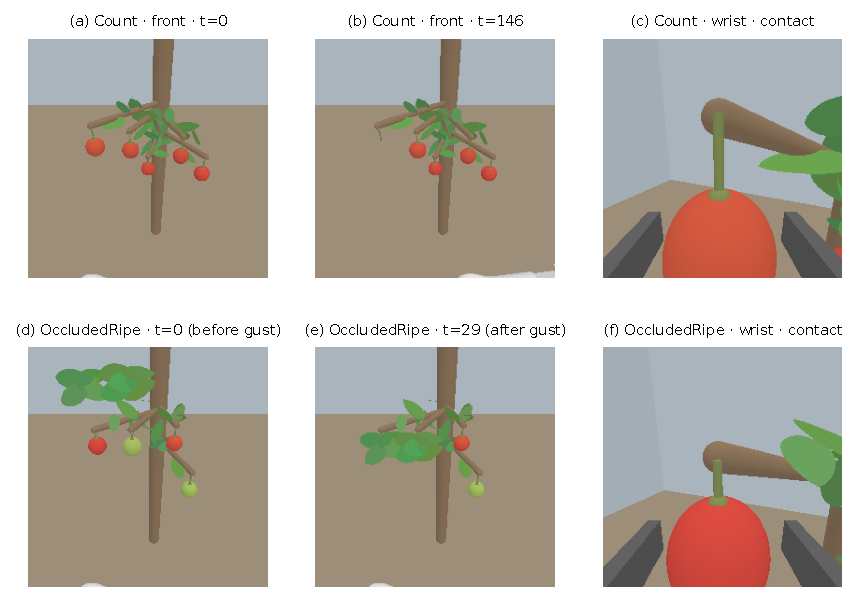
\includegraphics[width=0.78\linewidth]{fig2_scene}
\caption{\bench\ tasks. (a--c) FruitCount: front view at the start and after one pick, and the wrist view at contact. (d--f) FruitOccludedRipe: the front view before and after the wind gust (two leaf clusters now hide fruits) and the wrist view at contact.}
\label{fig:scene}
\end{figure}

\paragraph{Demonstrations} A scripted demonstrator plans with mplib \citep{mplib} through eight phases (observe, reach, approach, grasp, pull, carry, release, settle); failed attempts are discarded, and every frame stores the ground-truth fruit poses and attachment, visible pixels per camera, phase labels and TCP pose. Recovery demonstrations (DART-H, Section~\ref{sec:dart}) use the same demonstrator with execution noise. Table~\ref{tab:dataset} summarizes the 640 demonstrations. After the gust, the targeted fruits are fully invisible in the front camera; over all frames in which an occluded fruit is still on the tree, it is invisible in 72\% of frames on average (median 78\%), and two-thirds of the leaf clusters hide a ripe fruit (Table~S1 in the Supplementary material, with the phase structure).

\begin{table}[t]
\centering
\caption{Benchmark statistics (steps: mean $\pm$ SD). Acceptance: fraction of demonstrator attempts that succeeded. Training features: 88,607 samples (clean) and 173,791 (clean + DART-H).}
\label{tab:dataset}
\footnotesize
\begin{adjustbox}{max width=\textwidth}\begin{tabular}{llrccccc}
\toprule
Set (episodes) & Task & $n$ & Steps & Range & Fruits & Picks & Acceptance\\
\midrule
Clean train (0--99) & FruitCount & 100 & $474\pm124$ & 320--757 & 4.73 & 2.85 & 0.96\\
 & FruitOccludedRipe & 100 & $412\pm85$ & 295--710 & 4.69 & 2.54 & 0.98\\
DART-H train (100--199) & FruitCount & 100 & $455\pm133$ & 314--876 & 4.62 & 2.70 & 0.57\\
 & FruitOccludedRipe & 100 & $397\pm89$ & 297--672 & 4.78 & 2.46 & 0.66\\
Development (200--219) & FruitCount & 20 & $487\pm162$ & 321--766 & 5.05 & 3.10 & 1.00\\
 & FruitOccludedRipe & 20 & $369\pm71$ & 300--471 & 4.60 & 2.35 & 0.95\\
Validation (0--49) & FruitCount & 50 & $459\pm142$ & 314--904 & 4.58 & 2.82 & 0.98\\
 & FruitOccludedRipe & 50 & $396\pm87$ & 300--630 & 4.72 & 2.50 & 0.96\\
Validation (50--99) & FruitCount & 50$^{a}$ & $499\pm169$ & 322--1037 & 4.67 & 2.98 & 0.91\\
 & FruitOccludedRipe & 50 & $392\pm73$ & 304--534 & 4.54 & 2.52 & 0.98\\
\bottomrule
\end{tabular}\end{adjustbox}

\footnotesize $^{a}$Statistics over 49 episodes; the ground-truth file of one episode was regenerated after these statistics were computed.
\end{table}

\section{HarvestMem: event-centric memory for harvesting}
\label{sec:method}

\subsection{Design principles}
\label{sec:principles}
HarvestMem rests on four design principles.
\textbf{P1, index memory by events, not by time:} memory slots go to the contact and detachment of each pick, which time-indexed memory provably loses as operation lengthens (Section~\ref{sec:coverage}).
\textbf{P2, ground events in physics:} events are defined by the tool-to-fruit distance, which is measurable on a real robot, interpretable, and transferable across crops through one parameter commensurate with fruit size.
\textbf{P3, change what is remembered, not how much or how:} budget, tokens, architecture and inference cost of the base VLA are unchanged, and the same selection is used in training and deployment.
\textbf{P4, remember where before remembering what:} an event on a hidden fruit can be recognized only if the fruit was anchored while visible, so spatial memory is built first and drives episodic memory.
In the resulting system (Fig.~\ref{fig:overview}), \fdm\ (Section~\ref{sec:fdm}) builds the spatial memory and the distance $d_t$, a causal detector (Section~\ref{sec:events}) finds picking events, and \pekm\ (Section~\ref{sec:pekm}) chooses which $B$ past frames the VLA sees.

\subsection{Problem formulation and base policy}
\label{sec:formulation}
At decision time $t$, the policy $\pi_\theta$ receives the current front and wrist images $o_t$, the proprioceptive state $s_t$, the instruction $l$ and a memory $\mathcal{M}_t$ of past frames, and outputs an action chunk $A_t = (a_t,\dots,a_{t+H-1}) = \pi_\theta(o_t, s_t, l, \mathcal{M}_t)$ with $H=20$, of which the first 16 actions are executed before the next decision. The memory is the output of a selection function
\begin{equation}
\mathcal{M}_t = S\big(\{0,\dots,t\};\, d_{0:t}\big),\qquad |\mathcal{M}_t| = \min(B, t+1),
\label{eq:selection}
\end{equation}
that is \emph{causal} and \emph{budget-preserving} (exactly $B$ frames, as with uniform sampling), so any difference in behaviour is due to memory content rather than memory size.

The base policy is a memory-augmented VLA (MME-VLA, \tbd{cite base model}) in the $\pi_{0.5}$ family \citep{pi05_2025}: a PaliGemma backbone (Gemma-2B, \citealp{beyer2024paligemma}), a 300M-parameter action expert that generates action chunks by flow matching \citep{lipman2023flow}, and a 150M-parameter memory expert that attends over the $B=16$ selected frames, each encoded by the frozen SigLIP encoder \citep{zhai2023siglip} into 16 tokens. We initialize from a checkpoint trained on a general manipulation-memory benchmark (\tbd{cite RoboMME}) and fine-tune all non-vision parameters on \bench.

\subsection{Event signal and causal event detection}
\label{sec:signal}
\label{sec:events}
The event signal is
\begin{equation}
d_t = \min_{j \in \mathcal{P}_t} \lVert p^{\mathrm{TCP}}_t - c_j \rVert_2,
\label{eq:signal}
\end{equation}
where $p^{\mathrm{TCP}}_t$ is the TCP position from forward kinematics, $c_j$ the centre of fruit $j$, and $\mathcal{P}_t$ the set of fruits that are \emph{pickable and still attached} (all fruits in FruitCount, ripe fruits in FruitOccludedRipe). If $\mathcal{P}_t$ is empty, $d_t = 10$~m; a frame without a measurement is unknown. The signal falls below the fruit radius when the gripper encloses a fruit and jumps at detachment, because a detached fruit leaves $\mathcal{P}_t$. In training, $d_t$ comes from the simulator state; at deployment, from \fdm\ with the same definition.

A frame is \emph{near} if $d_t \le r$ and \emph{far} otherwise; an unknown frame inherits the last known state, so a dropped measurement neither starts nor ends an event. An \emph{event} is a maximal run of near frames $[t_s, t_e]$ and contributes two keyframes:
\begin{align}
t^{\mathrm{c}} &= \min\Big\{ f \in [t_s, \min(t_e, t)] : d_f \le \min_{t_s \le g \le \min(t_e,t)} d_g + \mathrm{tol} \Big\}, \label{eq:contact}\\
t^{\mathrm{r}} &= t_e + 1 \quad \text{(only if } t_e < t\text{)}. \label{eq:release}
\end{align}
The contact keyframe is the first frame within $\mathrm{tol}$ of the minimum distance of the run observed so far (the gripper settling around the fruit), and the release keyframe is the first far frame after the run (the detachment). We use $r=3$~cm, commensurate with the fruit radius and below half the inter-fruit spacing, and $\mathrm{tol}=5$~mm, both chosen on the training set. For noisy deployment signals, a \emph{hysteresis} variant enters an event at $d_t \le r$, leaves it only at $d_t > 1.5r$ and discards runs shorter than 3 frames, which suppresses chatter around the threshold without the delay of a median filter.

\subsection{Why time-indexed memory loses events: a coverage analysis}
\label{sec:coverage}
Let the key set $S_e$ of a completed pick $e$ be the frames within $\pm W$ of its contact and release keyframes, $|S_e| \le 2(2W+1)$; the pick is \emph{covered} at decision time $t$ if the memory holds a frame of $S_e$. Uniform memory keeps one frame every $\Delta_t = t/(B-1)$ frames. If the phase of this grid is independent of the timing of the pick, the expected number of memory frames in $S_e$ is $|S_e|/\Delta_t$, and when $\Delta_t$ exceeds each keyframe window, at most one memory frame falls in each window, so that
\begin{equation}
c_U(t) \approx \min\!\Big(1,\; \frac{(B-1)\,|S_e|}{t}\Big).
\label{eq:coverage}
\end{equation}
Two consequences are central to harvesting. First, \textbf{forgetting grows with operating time}: for a fixed budget, coverage decays as $1/t$, and the most recent pick enjoys no protection. Second, \textbf{budgets must grow linearly with time}: to keep coverage $c$, uniform memory needs $B \ge 1 + c\,t/|S_e|$; with $W=3$ ($|S_e|=14$) and $t=600$, full coverage would require about 44 frames, nearly three times the base model's budget, at a quadratically growing attention cost. Event indexing removes the dependence on $t$: with keyframe cap $k$, \pekm\ covers the $\lfloor k/2\rfloor$ most recent picks with probability one at every decision time, using a constant two slots per remembered pick. Section~\ref{sec:res_memory} shows that Eq.~(\ref{eq:coverage}) predicts the measured coverage of uniform memory to within 0.012 at every budget, and that \pekm\ keeps the most recent pick at all decision times.

\subsection{Picking-Event Keyframe Memory}
\label{sec:pekm}
Algorithm~\ref{alg:pekm} gives the selection rule: keyframes are taken from the most recent event backwards, contact before release, until at most $k$ are reserved, and the remaining $B-|\mathcal{K}|$ slots are filled at evenly spaced positions among the non-key frames, including the first and the last.

\begin{algorithm}[t]
\caption{PEKM selection at decision time $t$}
\label{alg:pekm}
\begin{algorithmic}[1]
\Require distances $d_{0:t}$, budget $B$, keyframe cap $k<B$, radius $r$, tolerance $\mathrm{tol}$
\If{$t+1 \le B$} \Return $\{0,\dots,t\}$ \EndIf
\State $\mathcal{E} \gets \textsc{DetectEvents}(d_{0:t}, r, \mathrm{tol})$ \Comment{Eqs.~(\ref{eq:contact})--(\ref{eq:release})}
\State $\mathcal{K} \gets \emptyset$
\For{$e \in \mathcal{E}$ from newest to oldest}
  \For{$f \in (t^{\mathrm{c}}_e, t^{\mathrm{r}}_e)$ if defined}
    \If{$|\mathcal{K}| < k$ and $f \notin \mathcal{K}$} $\mathcal{K} \gets \mathcal{K} \cup \{f\}$ \EndIf
  \EndFor
\EndFor
\State $R \gets \{0,\dots,t\} \setminus \mathcal{K}$ \Comment{sorted}
\State $U \gets \{R[\lfloor i\,(|R|-1)/(B-|\mathcal{K}|-1) \rfloor] : i = 0,\dots,B-|\mathcal{K}|-1\}$ \Comment{evenly spaced}
\State \Return $\mathrm{sort}(\mathcal{K} \cup U)$
\end{algorithmic}
\end{algorithm}

\paragraph{Properties} \pekm\ is a drop-in memory for a pretrained VLA. It is \emph{budget-preserving} ($|\mathcal{M}_t| = B$), so compute and latency are unchanged. It \emph{strictly nests the baseline}: with $k=0$ it is exactly the uniform sampling of the base model. It is \emph{causal}: an ongoing event contributes a provisional contact frame. It is \emph{train--deploy consistent}: every training memory is computed with the same function and signal definition as at deployment. It provides \emph{signal isolation}: $d_t$ selects frame indices but never enters the network, so a perception error can change \emph{which} frames are seen but cannot inject a wrong value into the policy. With $k=4$ the memory holds the keyframes of the two most recent picks, which show which fruit is gone and that a basket drop has occurred; $k=8$ covers four picks, enough for every FruitOccludedRipe episode and nearly every FruitCount episode.

\paragraph{Soft variant (PEKM-S)} As an alternative to hard reservation, PEKM-S samples frames from a density that mixes a uniform term with a proximity term over the $N$ history frames:
\begin{equation}
\rho_f = \frac{1-\alpha}{N} + \alpha \frac{w_f}{\sum_g w_g},\qquad w_f = \exp\!\Big(-\frac{d_f}{\tau_d}\Big),
\label{eq:soft}
\end{equation}
with $\tau_d=5$~cm. The per-frame density is capped at one slot by water-filling, and frames are drawn by systematic sampling of the cumulative density, so the selection is deterministic given $d_{0:t}$. The first frame and the 4 most recent uniform slots are always kept. The mixing weight $\alpha \in [0,1]$ interpolates between uniform memory ($\alpha=0$) and pure proximity memory ($\alpha=1$).

\subsection{SAM-based fruit distance module}
\label{sec:fdm}
On a real robot, $d_t$ must come from perception. \fdm\ produces it from the front RGB-D camera, forward kinematics and the gripper state in four steps.

\paragraph{(i) Colour-prompted segmentation} Ripe (red) and unripe (green) candidate regions are found by HSV thresholds and connected components (calibrated on training renders; pixel F1 0.986 and 0.976). Each component prompts SAM \citep{kirillov2023sam} with its bounding box padded by 2 pixels and its centroid as a positive point, keeping the mask with the highest predicted IoU. Masks much larger than their prompt region (e.g.\ a whole branch) or of mixed colour (purity $<0.3$) are rejected, duplicates are removed by mask non-maximum suppression, and ripeness is the dominant colour class inside the mask. The prompt design (2-pixel padding plus a point) was selected on training renders, where it gave an instance F1 of 0.991 and a mean IoU of 0.970.

\paragraph{(ii) Fruit anchors (spatial memory)} At the first frame, before any occlusion, every mask is back-projected with the depth image and camera parameters, and the fruit centre is the median visible surface point pushed back along the viewing ray by the fruit radius,
\begin{equation}
\hat c_j = \tilde p_j + \hat\rho_j \frac{\tilde p_j - o_{\mathrm{cam}}}{\lVert \tilde p_j - o_{\mathrm{cam}} \rVert},\qquad \hat\rho_j = \frac{z_j}{f_x}\sqrt{\frac{|m_j|}{\pi}},
\end{equation}
where $\tilde p_j$ is the median back-projected point of mask $m_j$, $z_j$ its median depth, $f_x$ the focal length and $o_{\mathrm{cam}}$ the camera centre; anchors closer than 3~cm are merged. Each anchor stores its centre and ripeness and persists whether or not the fruit remains visible, which is how the module remembers a ripe fruit that wind later hides. SAM therefore runs only once per episode.

\paragraph{(iii) Picked-fruit detection from two kinds of evidence} An anchor is marked \emph{picked} by either of two causal cues. \emph{Depth vacancy} (visual): the median depth around the anchor's projected surface point lies more than 5~cm behind the expected surface for 3 consecutive frames (more than 2~cm in front means occluded, and the anchor is left unchanged). \emph{Grasp holding} (proprioceptive): the gripper is commanded closed but the fingers stop between the empty-closed and open positions for 2 frames while the TCP is within $r$ of an unpicked anchor. Vacancy needs no contact sensing but is blind while the arm occludes the anchor during carrying; grasp holding fires exactly at detachment.

\paragraph{(iv) Distance} $\hat d_t$ is the distance from the TCP to the nearest unpicked pickable anchor, exactly as in Eq.~(\ref{eq:signal}), and feeds the hysteresis detector and \pekm. Through this scalar interface, SAM can be replaced by any detector (e.g.\ YOLO-seg or a crop-specific network) without retraining the policy.

\subsection{Phase-aware recovery demonstrations (DART-H)}
\label{sec:dart}
\label{sec:training}
Imitation policies drift away from the demonstrated states in closed loop \citep{ross2011dagger}. Following DART \citep{laskey2017dart}, we inject noise while the demonstrator executes but record its clean actions, replanned from the perturbed state, as labels that show how to recover. Two choices adapt DART to harvesting. First, white joint noise is filtered out by the position controller, so we use \emph{temporally correlated} Ornstein--Uhlenbeck noise on the seven joint targets,
\begin{equation}
\epsilon_{t+1} = \epsilon_t - \frac{\epsilon_t}{\tau} + \sigma\sqrt{\frac{2}{\tau}}\,\xi_t,\qquad \xi_t \sim \mathcal{N}(0, I),
\end{equation}
with $\sigma=0.04$~rad and $\tau=10$ steps, which produces median TCP displacements of 2.50~cm (FruitCount) and 2.54~cm (FruitOccludedRipe), the scale of the drift observed in closed loop. Second, the noise is \emph{phase-gated}: scaled by 1 in reach, pull and carry, 0.5 in approach, and 0 in observe, grasp, release and settle, so grasping and releasing, where a perturbation would mostly produce failed attempts, stay clean. Failed perturbed attempts are discarded as for clean demonstrations (acceptance 0.57 in FruitCount and 0.66 in FruitOccludedRipe), and the training set combines 200 clean and 200 DART-H episodes.

\paragraph{Training} All memory conditions are fine-tuned with identical settings and differ only in the keyframe cap $k$ used to compute the memory of each training sample: 12{,}000 steps; global batch size 64; AdamW with gradient clipping at 1.0; 500 warm-up steps to a peak learning rate of $2.5\times10^{-5}$, then cosine decay to $2.5\times10^{-6}$; EMA decay 0.999; frozen vision encoder; seed 42. Normalization statistics are recomputed on \bench\ because the RM75-B joint ranges differ from those of the pretraining robot. Each condition is trained with fully sharded data parallelism on four NVIDIA L20 (48~GB) GPUs.

\section{Experimental design}
\label{sec:design}

\subsection{Research questions and experiment map}
The experiments address eight research questions (Table~\ref{tab:rq}). E1--E6 and E9--E11 analyse the components offline and in perception; E7 and E8 evaluate closed-loop harvesting under the pre-registered protocol of Section~\ref{sec:protocol}.

\begin{table}[t]
\centering
\caption{Research questions and experiment map. C1--C5: contributions in Section~\ref{sec:intro}.}
\label{tab:rq}
\footnotesize
\setlength{\tabcolsep}{3pt}
\begin{adjustbox}{max width=\textwidth}\begin{tabular}{>{\raggedright\arraybackslash}p{1.45cm}>{\raggedright\arraybackslash}p{4.5cm}>{\raggedright\arraybackslash}p{3.2cm}>{\raggedright\arraybackslash}p{3.4cm}>{\raggedright\arraybackslash}p{1.0cm}}
\toprule
Exp. (RQ) & Question & Data & Main metrics & Contr.\\
\midrule
E1 (RQ1) & Do the tasks require memory; how strong is the occlusion? & 640 demonstrations & Steps, picks, occlusion & C1\\
E2 (RQ2) & Does the tool-to-fruit distance locate picks; how sensitive is it to $r$, tol? & Train 200 (selection), val 199, DART-H 200 & Event P/R/F1, count exact, keyframe timing & C2\\
E3 (RQ3) & How robust are events and memory to noise, dropout and bias? & Val 199, 5 seeds per level & Event F1, count exact, keyframe recall & C2, 3\\
E4 (RQ4) & What do uniform memory and \pekm\ retain; does the coverage model hold? & Val 199--200, 5318 decisions & Event coverage, count recoverability, recency, gap & C2\\
E5 (RQ5) & Can SAM segment fruits and ripeness under occlusion and lighting shifts? & 8644 rendered images with GT masks & Instance F1, IoU, recall by visibility, latency & C3\\
E6 (RQ6) & Does RGB-D $\rightarrow$ \fdm\ $\rightarrow$ events reproduce the GT memory? & Val 199 RGB-D + proprioception & Anchor/distance error, event F1, memory agreement & C3\\
E7 (RQ7) & Does event memory improve closed-loop harvesting? & Val 50--99 $\times$ 3 seeds & Success, completion, wrong/over-pick, drop & C2, 5\\
E8 (RQ7) & Is the gain due to event information? & As E7 & Paired differences to EV & C2, 3, 5\\
E9 (RQ8) & Where do policies fail in closed loop; does DART-H help? & 10 episodes per set; E7 & TCP error by horizon; C0 vs K0 & C4\\
E10 (--) & Generalization and supporting evidence & Unseen layouts; memory benchmark & Success by quota; ablations & C2\\
E11 (RQ8) & What does the approach cost at run time? & CPU / L20 GPU & Selection and SAM latency & C2, 3\\
\bottomrule
\end{tabular}\end{adjustbox}
\end{table}

\subsection{Data and splits}
\label{sec:splits}
Training, validation and test seeds are drawn from disjoint seed ranges (base seeds 100000, 200000 and 300000), so every evaluated layout is unseen during training. All parameters of the method (Table~\ref{tab:provenance}) were fixed on training data or by physical reasoning, never on validation data. Validation episodes 0--49 were used in earlier development evaluations; the formal closed-loop evaluation (E7, E8) therefore uses validation episodes 50--99, which had not been used for any evaluation or tuning. A separate development set (episodes 200--219 of the training seed range) serves only as a go/no-go gate before the formal runs. The perception set for E5 replays validation episodes 0--49 of both tasks and renders front and wrist RGB-D images with ground-truth instance segmentation every 10th frame (4322 time steps, 8644 images); we verified that replay reproduces the recorded episodes by comparing the rendered and recorded RGB. HSV thresholds and SAM prompt settings were calibrated on 20 rendered training episodes. The offline analyses on validation demonstrations use 199 of the 200 episodes: the ground-truth file of one episode was unreadable and was regenerated afterwards from its recorded seed, with identical joint trajectories, and the coverage-by-time analysis, run after the regeneration, uses all 200.

\begin{table}[t]
\centering
\caption{Provenance of all method parameters. No parameter was tuned on validation or test data.}
\label{tab:provenance}
\footnotesize
\begin{adjustbox}{max width=\textwidth}\begin{tabular}{>{\raggedright\arraybackslash}p{4.2cm}>{\raggedright\arraybackslash}p{2.9cm}>{\raggedright\arraybackslash}p{6.0cm}}
\toprule
Parameter & Value & Source\\
\midrule
Memory budget $B$ & 16 frames & Fine-tuning configuration of the base model\\
Keyframe cap $k$ & 4, 8 & Training-set event counts (at most 3 / 5 picks per episode)\\
Event radius $r$, tolerance tol & 3 cm, 5 mm & Training-set sensitivity (E2); fruit radius 2.5--2.9 cm\\
Hysteresis exit, minimum run & $1.5r$, 3 frames & Fixed a priori\\
Coverage window & $\pm3$ frames & Fixed a priori (matching window of E2)\\
PEKM-S $\tau_d$, recent slots & 5 cm, 4 & Fixed a priori\\
DART-H $\sigma$, $\tau$, phase scales & 0.04 rad, 10, (1, 0.5, 1, 1) & Calibration on training generation: TCP displacement $\approx$2.5 cm\\
HSV thresholds & pixel-level calibration & Pixel F1 on 20 rendered training episodes\\
SAM prompt (box pad, point) & 2 px, centroid & Instance F1 on rendered training episodes\\
Vacancy / occlusion margins & 5 cm / 2 cm, 3 frames & Physical scale (fruit diameter $\approx$5 cm)\\
Grasp cue & 2 frames, within $r$ & Gripper geometry (empty-closed vs open)\\
Training (steps, batch, LR, EMA) & 12k, 64, $2.5\times10^{-5}$, 0.999 & Base-model fine-tuning recipe, unchanged\\
\bottomrule
\end{tabular}\end{adjustbox}
\end{table}

\subsection{Compared methods}
\label{sec:baselines}
\paragraph{Memory selection (E4, E7, E8)} All memories have exactly $B$ frames:
\begin{itemize}
\item \textbf{Uniform (U, K0)}: the base model's even sampling over frames 0 to $t$, identical to \pekm\ with $k=0$;
\item \textbf{Recent}: the last $B$ frames (sliding window);
\item \textbf{Random}: frame 0, frame $t$ and $B-2$ random frames (5 seeds);
\item \textbf{\pekm\ (K$k$)}: $k \in \{2, 4, 8, 12\}$ offline, $k \in \{4, 8\}$ trained for closed loop;
\item \textbf{PEKM-S}: the soft variant of Eq.~(\ref{eq:soft}), $\alpha \in \{0.25, 0.5, 1.0\}$.
\end{itemize}

\paragraph{Counterfactual controls (E8)} A change of memory content can affect a policy simply because the frames are different, whatever information they carry. To separate the two effects, each event memory (EV) is compared at test time with three controls that keep the budget, the first frame and the recent window: \textbf{EVU}, the same sampler driven by a uniform density, i.e.\ the procedure without event information; \textbf{EVR}, uniform memory in which exactly the frames that EV dropped are replaced by the same number of random non-uniform frames; and \textbf{EVA}, the anti-event selection driven by $1-w_f$ (frames far from fruits). Only EV$-$EVU and EV$-$EVR differences that favour EV, with EVA no better than U, are interpreted as an effect of event information.

\paragraph{Event detectors (E2, E3, E6)} Plain thresholding (Section~\ref{sec:events}), a causal 5-frame median filter followed by thresholding (median5), and hysteresis with a 3-frame minimum run.

\paragraph{Fruit segmentation (E5)} \textbf{HSV}, colour thresholds and connected components, a traditional baseline; \textbf{SAM-AUTO}, automatic SAM masks filtered by colour and compactness, i.e.\ zero-shot SAM without prompts (ViT-B and ViT-H, every 5th frame); \textbf{\fdm}, colour-prompted SAM with ViT-B, ViT-L and ViT-H backbones; and \textbf{SAM-GTBOX}, SAM prompted with the ground-truth box, an upper bound on mask quality given a correct prompt.

\paragraph{Perception chain (E6)}
\begin{itemize}
\item \textbf{GT}: the simulator distance, an upper bound;
\item \textbf{\fdm}: frame-0 anchors with depth and grasp evidence;
\item \textbf{\fdm\ + noisy depth}: depth noise $\sigma(z) = 1~\mathrm{mm} + 2.5~\mathrm{mm}\cdot z^2$ ($z$ in m) and 2\% missing pixels, typical of consumer RGB-D cameras;
\item \textbf{Depth-only}: no grasp evidence;
\item \textbf{Post-gust anchors}: anchors built at frame 29, after the wind gust, i.e.\ without spatial memory acquired before occlusion;
\item \textbf{Per-frame}: no anchors; the current frame's colour detections are back-projected, and an invisible fruit is unknown.
\end{itemize}

\paragraph{Training data (E9)} C0 is trained on clean demonstrations only and compared with K0, trained on clean plus DART-H demonstrations; both use uniform memory and identical settings.

\subsection{Metrics}
\label{sec:metrics}
\paragraph{Closed-loop harvesting (E7, E8)} The primary metric is the \textbf{success rate}, with the task-specific success conditions of Section~\ref{sec:tasks}. Process metrics are the \textbf{harvest completion} (fruits correctly in the basket divided by the target number), the \textbf{wrong-pick rate} (episodes with an unripe fruit in the basket, FruitOccludedRipe), the \textbf{over-pick rate} (episodes with more than $N$ fruits in the basket, FruitCount), the \textbf{drop rate} (episodes in which a fruit is dropped outside the basket) and the steps to completion and per pick. Episodes terminated by infrastructure faults are reported separately as the \textbf{engineering-error rate} and are not counted as policy failures.

\paragraph{Events (E2, E3, E6)} A detected event $[t_s, t^{\mathrm{r}}]$ is matched one-to-one, in time order, to a ground-truth detachment (the first frame at which the fruit is no longer attached) if the detachment falls within $[t_s-3, t^{\mathrm{r}}+3]$. We report precision, recall and F1; the \textbf{count exact rate}, the fraction of episodes in which the number of detected events equals the number of picks; and the contact lead and release error, in frames relative to detachment.

\paragraph{Memory (E3, E4, E6)} Memories are evaluated at every decision point (every 16 frames). A completed pick is \emph{covered} if the memory holds a frame within $\pm 3$ frames of its contact or release keyframe. We report:
\begin{itemize}
\item \textbf{event coverage}: the fraction of completed picks that are covered;
\item \textbf{run coverage}: at least one frame inside the pick's near run;
\item \textbf{count recoverability}: the fraction of decisions at which every completed pick is covered, i.e.\ the memory suffices in principle to count the picks;
\item \textbf{recency coverage}: coverage of the last, second-last and third-last pick;
\item the near-frame fraction and the median gap between memory frames, as the cost in temporal coverage;
\item for perturbed or perceived signals, the Jaccard similarity to the GT memory and the recall of GT keyframes within $\pm3$ frames.
\end{itemize}

\paragraph{Perception (E5, E6)} Segmentation is scored by instance precision, recall and F1 at IoU $\ge 0.5$, with fruits of fewer than 20 (front) or 60 (wrist) visible pixels treated as ignore regions; by the mean IoU and ripeness accuracy of matched instances; by recall stratified by the visible fraction of the fruit ($>$75\%, 25--75\%, $<$25\%); and by latency per image on an L20 GPU. Illumination robustness is measured by re-rendering every third frame photometrically as overcast or dusk, direct sun and warm low sun, with the colour thresholds kept as calibrated. Anchors are scored by recall and precision against the true fruit positions at frame 0 (5~cm gate), median and 90th-percentile localization error, ripeness accuracy, and the fraction of leaf-hidden ripe fruits that have an anchor; distances by the error of $\hat d_t$ in the near range ($d_t \le 10$~cm).

\subsection{Closed-loop evaluation protocol}
\label{sec:protocol}
The closed-loop protocol was written and sealed (SHA-256 digest recorded) before the formal runs, and the first completed run is the result, without re-runs or selection.
\begin{itemize}
\item \textbf{Episodes and seeds.} Validation episodes 50--99 of each task are evaluated with three policy sampling seeds (7, 8, 9), giving 150 trials per task and condition. A decision is made every 16 steps, and an episode ends at success, failure or 1300 steps.
\item \textbf{Conditions.} K0, K4 and K8 (uniform and \pekm, all trained on clean plus DART-H data) and C0 (uniform, clean data only).
\item \textbf{Pairing.} For each episode and seed, all conditions run in one block with the same environment seed and initial state, in randomized order, on policy servers whose identity is logged; each server holds a fixed group of conditions so that their checkpoints fit in GPU memory.
\item \textbf{Validity gates.} A run is valid only if engineering errors are at most 2\% of trials, every block is complete, and a per-decision audit confirms that the frame indices fed to the model equal those recomputed offline by the declared selection rule from the logged signal.
\item \textbf{Development gate.} Before the formal run, K0 is evaluated on the development set; the formal evaluation proceeds only if its success rate exceeds 5\% and engineering errors are at most 2 episodes, so a broken pipeline cannot consume the validation episodes.
\end{itemize}

\subsection{Statistical analysis}
\label{sec:stats}
Differences between conditions are estimated as paired differences in success rate. Confidence intervals come from a cluster bootstrap that resamples episodes and keeps all seeds and conditions of an episode together (20{,}000 resamples, fixed random seed). The primary contrasts are K4$-$K0 and K8$-$K0 per task, and the family of primary tests is corrected by the Holm method \citep{holm1979simple}. We report 95\% confidence intervals for differences, and a difference is called \emph{equivalent} if its 90\% confidence interval lies within $\pm\delta$ with $\delta=12$ percentage points (two one-sided tests, \citealp{schuirmann1987tost}). Secondary contrasts (DART-H: K0$-$C0; counterfactual controls) are reported with unadjusted intervals and labelled as secondary. Offline experiments (E2--E6) are deterministic given the data, except for noise and random baselines, which use 5 seeds; we report means over seeds.

\subsection{Hyperparameter provenance and implementation}
\label{sec:provenance}
To prevent tuning on evaluation data, every parameter was fixed before the formal evaluation, either on training data or from physical or architectural considerations (Table~\ref{tab:provenance}). The simulation uses ManiSkill3 \citep{tao2025maniskill3} with SAPIEN rendering and mplib \citep{mplib} motion planning. The policy is implemented in JAX on the openpi code base \citep{black2024pi0}, and SAM in PyTorch with the official checkpoints. Experiments ran on a server with eight NVIDIA L20 (48~GB) GPUs; in closed-loop evaluation, policy servers run on GPUs separate from the simulators.

\section{Results}
\label{sec:results}

\subsection{The benchmark requires memory (RQ1)}
\label{sec:res_bench}
Episodes last 300 to 1000 control steps with 2--5 picks (Table~\ref{tab:dataset}), while a pick, from contact to detachment, occupies only about a dozen frames. A leaf-hidden fruit is invisible in a median 78\% of the frames in which it still hangs on the tree, two-thirds of the hidden fruits are ripe, and in FruitCount the basket is never in the front view. Neither task can be solved from the current frame: the policy must remember where hidden ripe fruits are and how many fruits it has picked.

\subsection{Picking events from the tool-to-fruit distance (RQ2, RQ3)}
\label{sec:res_events}
\label{sec:res_robust}
\emph{Detection is exact over a physically determined plateau.} Events detected from the ground-truth distance have precision, recall and F1 of exactly 1.000 for every radius between 1 and 4~cm, on the training set (where $r$ was selected) and the validation set, with the correct pick count in every validation episode (Fig.~\ref{fig:events}a; all radii in Supplementary Table~S2). At 0.5~cm the gripper does not always come that close (recall 0.628); beyond half the inter-fruit spacing, approaches to neighbouring fruits merge into spurious events (count exact 0.49 at 10~cm). The contact keyframe precedes detachment by a median of 4 frames and the release keyframe coincides with it. On the 200 perturbed DART-H demonstrations, precision is 0.998, recall 1.000 and the count is exact in 99\% of episodes.

\emph{Robustness yields an accuracy specification for perception.} Table~\ref{tab:robust} and Fig.~\ref{fig:events}b--d report detection on corrupted validation distances (5 seeds per level): white Gaussian noise, correlated Ornstein--Uhlenbeck noise, independent and contiguous dropouts (runs averaging 10 frames) and a constant bias. Independent dropouts are nearly harmless (F1 1.000 with 30\% of frames missing, since unknown frames inherit the last state), and a bias of $-1$ to $+2$~cm, as from a miscalibrated depth camera, leaves the count exact. White noise is the main threat: at 1~cm the plain detector's F1 falls to 0.846 and the count is exact in only 37\% of episodes, because the distance chatters around the threshold. Both filters remove this (F1 0.999, count exact 99\%); hysteresis does so without delay, keeping 0.995 of the K4 keyframes against 0.980 for the median filter, and is more robust to correlated noise (F1 0.953 versus 0.941 at 2~cm), so it is the default deployment detector. Long contiguous dropouts covering a whole approach remain the weak case (F1 0.894--0.913). With hysteresis, distance errors of up to 1.5~cm white noise (F1 0.987) or 2~cm correlated noise (F1 0.953) keep the event F1 above 0.95: this is the accuracy specification for any perception module that feeds \pekm.

\begin{table}[t]
\centering
\caption{Robustness of event detection and K4 memory to perturbations of the validation distance signal (5 seeds per level). Each cell: plain / median5 / hysteresis. Keyframe recall: fraction of clean-signal keyframes found within $\pm3$ frames in the perturbed memory.}
\label{tab:robust}
\footnotesize
\begin{adjustbox}{max width=\textwidth}\begin{tabular}{llccc}
\toprule
Perturbation & Level & Event F1 & Count exact & Keyframe recall (K4)\\
\midrule
None & -- & 1.000 / 1.000 / 1.000 & 1.00 / 1.00 / 1.00 & 1.000 / 1.000 / 1.000\\
White noise & 0.5 cm & 0.971 / 1.000 / 1.000 & 0.86 / 1.00 / 1.00 & 0.985 / 0.989 / 0.997\\
White noise & 1 cm & 0.846 / 0.999 / 0.999 & 0.37 / 0.99 / 0.99 & 0.932 / 0.980 / 0.995\\
White noise & 2 cm & 0.635 / 0.969 / 0.947 & 0.03 / 0.85 / 0.78 & 0.846 / 0.966 / 0.958\\
Correlated (OU) & 2 cm & 0.887 / 0.941 / 0.953 & 0.58 / 0.74 / 0.79 & 0.918 / 0.926 / 0.931\\
Independent dropout & 30\% & 1.000 / 1.000 / 0.998 & 1.00 / 1.00 / 0.99 & 0.998 / 0.999 / 0.996\\
Independent dropout & 50\% & 0.996 / 0.996 / 0.988 & 0.98 / 0.98 / 0.94 & 0.982 / 0.987 / 0.973\\
Contiguous dropout & 30\% & 0.913 / 0.913 / 0.894 & 0.62 / 0.62 / 0.55 & 0.882 / 0.901 / 0.867\\
Bias & $-1$ cm & 1.000 / 1.000 / 1.000 & 1.00 / 1.00 / 1.00 & 0.998 / 0.999 / 0.999\\
Bias & $+2$ cm & 1.000 / 1.000 / 1.000 & 1.00 / 1.00 / 1.00 & 1.000 / 1.000 / 1.000\\
\bottomrule
\end{tabular}\end{adjustbox}
\end{table}

\begin{figure}[t]
\centering
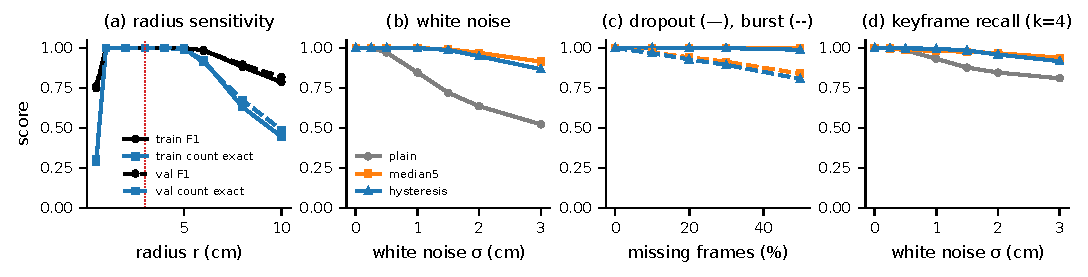
\includegraphics[width=\linewidth]{fig6_event_detection}
\caption{Event detection. (a) F1 and count exact rate versus radius $r$ (training and validation). (b) F1 versus white-noise level for the plain, median5 and hysteresis detectors. (c) F1 versus the fraction of missing frames, independent (solid) and contiguous (dashed). (d) Recall of K4 memory keyframes ($\pm3$ frames) versus white-noise level.}
\label{fig:events}
\end{figure}

\subsection{What a fixed-budget memory retains (RQ4)}
\label{sec:res_memory}
Table~\ref{tab:coverage} compares memories at the 16-frame budget over 5318 decision points of the validation demonstrations, and Fig.~\ref{fig:timeline} shows, for one episode, which frames each memory actually holds.

\emph{Uniform memory loses picks systematically.} It covers only 57.0\% of the completed picks, only 43.1\% of decisions can count the picks from memory, and even the most recent pick is covered in only 67.5\% of decisions. Keeping one frame every 30 frames while a pick lasts about a dozen, it retains picks by chance, like random memory (43.2\%); a recent-frame window is worse still (8.0\%). Figure~\ref{fig:timeline} makes the mechanism visible. In the first FruitCount validation episode (four picks, not selected for illustration), the even grid of uniform memory happens to fall on picks 2 and 4 but passes between the contact and release keyframes of picks 1 and 3. At the last decision the memory therefore holds evidence of only two of the four picks, and the number of fruits already in the basket cannot be recovered from it.

\begin{figure}[t]
\centering
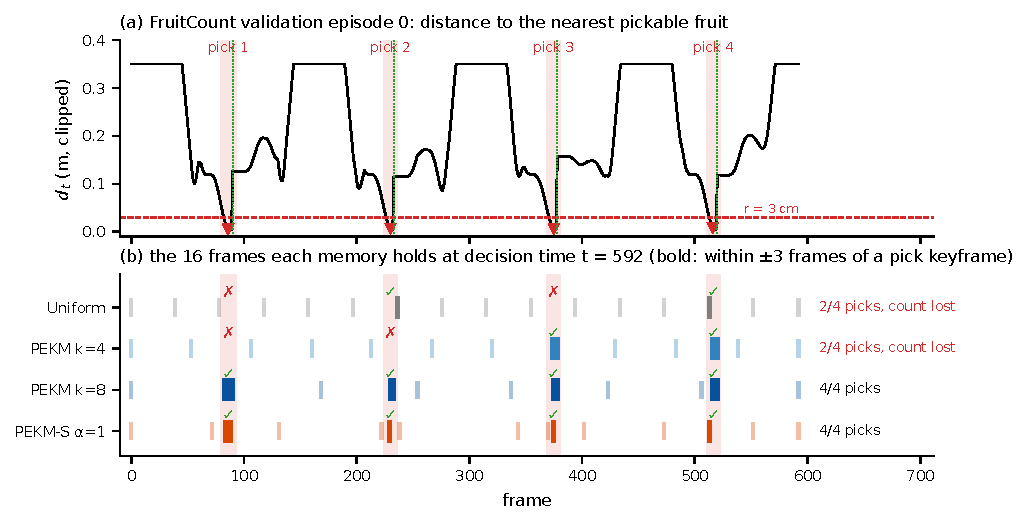
\includegraphics[width=\linewidth]{fig4_memory_timeline}
\caption{What a 16-frame memory actually holds. (a) TCP-to-fruit distance $d_t$ in the first FruitCount validation episode (four picks), with the detected picks and their $\pm3$-frame key windows (shaded), contact keyframes (triangles), the radius $r$ (dashed) and fruit detachments (dotted). (b) The frames held by each memory at the last decision ($t=592$); bold ticks lie within $\pm3$ frames of a contact or release keyframe, and \textcolor{green!50!black}{\checkmark}\,/\,\textcolor{red}{$\times$} marks whether each pick is covered. Uniform memory keeps picks 2 and 4 only because its grid happens to fall on them and misses picks 1 and 3, so the pick count is lost; \pekm\ with $k=4$ keeps the two most recent picks by construction, and $k=8$ and PEKM-S keep all four. Further examples are given in Supplementary Fig.~S1.}
\label{fig:timeline}
\end{figure}

\emph{Forgetting grows with operating time, as the coverage analysis predicts.} Over the 200 validation episodes (7884 decision--pick pairs), uniform memory at $B=16$ covers 97.8\% of completed picks in the first 200 frames, then 56.6\%, 40.8\% and only 26.4\% beyond 600 frames, and the most recent pick falls from 97.8\% to 21.7\% (Fig.~\ref{fig:theory}a,b). Equation~(\ref{eq:coverage}) predicts the measured coverage to within 0.012 at every budget (predicted / measured: 0.282 / 0.270 for $B=8$, 0.562 / 0.570 for $B=16$, 0.882 / 0.883 for $B=32$) and tracks its decay over time (Fig.~\ref{fig:theory}c): the failure is structural and cannot be tuned away. \pekm\ removes the dependence on time: $k=4$ and $k=8$ cover the most recent pick at every decision time, and $k=8$ covers at least 94.6\% of all completed picks even beyond 600 frames.

\begin{figure}[t]
\centering
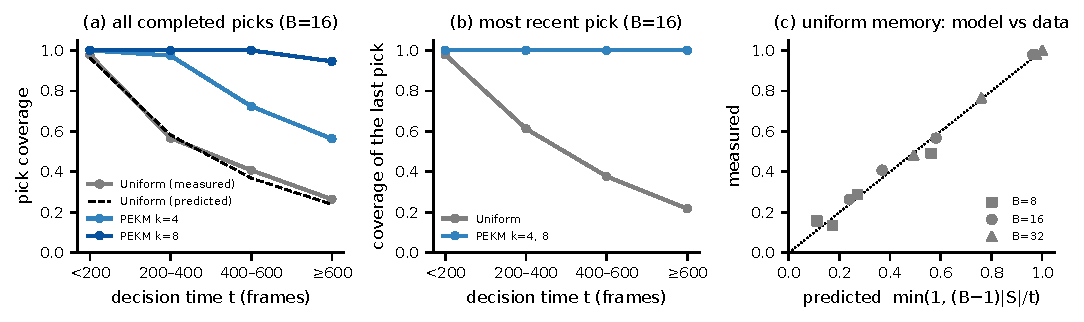
\includegraphics[width=\linewidth]{fig_coverage_theory}
\caption{Time-indexed memory forgets more the longer the robot works. (a) Coverage of all completed picks versus decision time at $B=16$: uniform memory (measured and predicted by Eq.~(\ref{eq:coverage})) and PEKM. (b) Coverage of the most recent pick. (c) Predicted versus measured coverage of uniform memory for every budget and decision-time bin.}
\label{fig:theory}
\end{figure}

\emph{\pekm\ retains recent picks by construction, without losing temporal context.} With $k=4$ the last two picks are always covered (picks 3 and 4 in Fig.~\ref{fig:timeline}) and overall coverage rises to 87.6\%; with $k=8$ coverage reaches 99.6\% and count recoverability 99.2\% (from 0.389 to 0.985 in FruitCount, from 0.485 to 1.000 in FruitOccludedRipe). The median gap between memory frames grows only from 14 to 17 frames (Fig.~\ref{fig:coverage}c). The soft variant concentrates six times more frames near fruits than U and covers older picks evenly, but at the cost of the most recent pick (0.814) and of temporal context (median gap 63 frames), which is why hard reservation is the main method. Increasing the cap to $k=12$ covers every pick, and an intermediate mixing weight ($\alpha=0.5$) trades the two effects without removing either (Table~\ref{tab:coverage}). \emph{Budget efficiency} follows: K4 with 8 frames (85.9\%) exceeds uniform memory with 16 frames and approaches it with 32 (88.3\%), and K8 with 16 frames (99.6\%) exceeds uniform memory with 32 (Fig.~\ref{fig:coverage}a), i.e.\ the same event information with a memory two to four times shorter.

\begin{table}[t]
\centering
\caption{Information retained by 16-frame memories (validation, both tasks; 5318 decisions, 7841 decision--pick pairs). Run cov.: at least one memory frame inside the pick's near run. Last / 2nd / 3rd: coverage of the most recent, second and third most recent pick. Near: fraction of memory frames with $d_t \le r$. Gap: median gap between memory frames (frames).}
\label{tab:coverage}
\footnotesize
\begin{adjustbox}{max width=\textwidth}\begin{tabular}{lcccccccc}
\toprule
Memory & Event cov. & Run cov. & Count rec. & Last & 2nd & 3rd & Near & Gap\\
\midrule
Uniform (U, K0) & 0.570 & 0.461 & 0.431 & 0.675 & 0.472 & 0.416 & 0.042 & 14\\
Recent & 0.080 & 0.069 & 0.046 & 0.145 & 0.000 & 0.000 & 0.049 & 209\\
Random & 0.432 & 0.364 & 0.329 & 0.533 & 0.351 & 0.231 & 0.040 & 41\\
PEKM $k=2$ & 0.729 & 0.681 & 0.579 & 1.000 & 0.430 & 0.336 & 0.085 & 17\\
\textbf{PEKM $k=4$} & \textbf{0.876} & \textbf{0.875} & \textbf{0.814} & \textbf{1.000} & \textbf{1.000} & 0.136 & 0.110 & 17\\
\textbf{PEKM $k=8$} & \textbf{0.996} & \textbf{0.995} & \textbf{0.992} & \textbf{1.000} & \textbf{1.000} & \textbf{1.000} & 0.123 & 17\\
PEKM $k=12$ & 1.000 & 1.000 & 1.000 & 1.000 & 1.000 & 1.000 & 0.124 & 17\\
PEKM-S $\alpha=0.5$ & 0.878 & 0.854 & 0.756 & 0.811 & 0.982 & 0.948 & 0.153 & 31\\
PEKM-S $\alpha=1$ & 0.897 & 0.873 & 0.770 & 0.814 & 1.000 & 1.000 & 0.265 & 63\\
\bottomrule
\end{tabular}\end{adjustbox}
\end{table}


\begin{figure}[t]
\centering
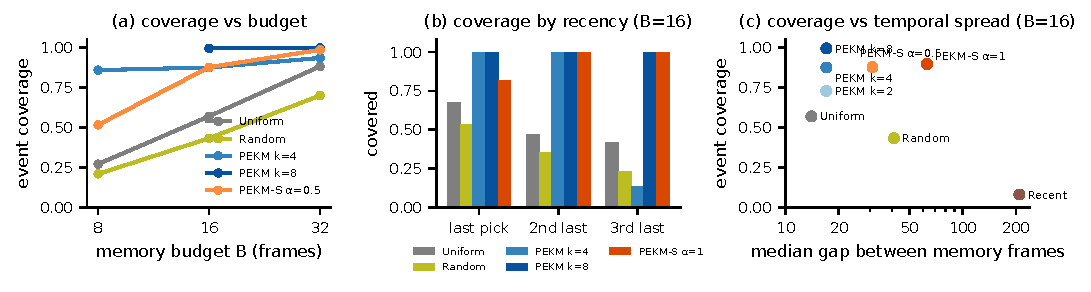
\includegraphics[width=\linewidth]{fig7_memory_coverage}
\caption{Memory coverage. (a) Event coverage versus budget $B$. (b) Coverage of the last three picks at $B=16$. (c) Event coverage versus median gap between memory frames: PEKM raises coverage without sacrificing temporal resolution.}
\label{fig:coverage}
\end{figure}

\subsection{Fruit segmentation with SAM (RQ5)}
\label{sec:res_sam}
Table~\ref{tab:sam} and Fig.~\ref{fig:sam} compare fruit segmentation on 8644 rendered validation images (13{,}424 front-camera and 4877 wrist-camera instances).

\emph{Prompted SAM gives the most accurate masks.} \fdm\ reaches an instance F1 of 0.991 (front) and 0.983--0.984 (wrist), with tighter masks than colour thresholding (IoU 0.974--0.978 versus 0.945), which matters because fruit centres are estimated from the mask, and recovers more partially hidden fruits (recall 0.967--0.976 versus 0.952 at 25--75\% visibility, 0.633--0.688 versus 0.615 below 25\%). Ripeness is correct for every matched instance with all methods.

\emph{Prompts are essential, and a small backbone suffices.} Without prompts, SAM-AUTO is precise (0.994--0.996) but misses partially hidden fruits (recall 0.57--0.62 at 25--75\% visibility, 0.21--0.26 below 25\%) and is four to seven times slower (395--626~ms per image). The three \fdm\ backbones have the same F1 (0.991) and differ by at most 0.004 in IoU, while latency grows from 94~ms (ViT-B) to 309~ms (ViT-H); since SAM runs once per episode, ViT-B is the practical choice for embedded platforms. With ground-truth boxes, SAM reaches F1 0.999 and a recall of 0.899 below 25\% visibility, so the remaining gap lies in prompting barely visible fruits, not in SAM's masks.

\emph{Illumination locates the component that must adapt.} We re-rendered every third frame under overcast or dusk, direct sun and warm low sun with the colour thresholds kept as calibrated (Table~\ref{tab:light}; Fig.~\ref{fig:sam}c), using a gamma-darkened ($0.55\,x^{1.2}$), a brightened ($1.35\,x^{0.85}$) and a warm colour cast (channel gains 1.12 / 1.00 / 0.80). Given correct box prompts, SAM's F1 stays at 0.999 and its IoU at 0.979 under all three conditions, whereas fixed colour thresholds do not transfer (F1 below 0.1) and \fdm\ inherits this through its prompts. The component to adapt for field use is therefore the prompt generator, which can be replaced by an illumination-normalized colour model or a learned detector without changing SAM, the anchors or the policy. \tbd{Optional: colour-normalized or learned prompt source as an additional row.}

\begin{table}[t]
\centering
\caption{Fruit instance segmentation and ripeness on rendered validation images (8644 images; 13{,}424 front and 4877 wrist instances). F1 at IoU $\ge 0.5$. IoU: mean over matched front-camera instances. R (vis.): front-camera recall by visible fraction (418 instances at 25--75\%, 109 below 25\%). Latency: median per front image on one L20 GPU. SAM-AUTO was evaluated on every 5th frame.}
\label{tab:sam}
\footnotesize
\begin{adjustbox}{max width=\textwidth}\begin{tabular}{llccccccc}
\toprule
Method & Backbone & F1 front & F1 wrist & IoU & R (25--75\%) & R ($<$25\%) & Ripeness & ms/img\\
\midrule
HSV thresholds & -- & 0.990 & 0.980 & 0.945 & 0.952 & 0.615 & 1.000 & 1.4\\
SAM-AUTO & ViT-B & 0.937 & 0.983 & 0.979 & 0.573 & 0.263 & 1.000 & 395\\
SAM-AUTO & ViT-H & 0.941 & 0.981 & 0.970 & 0.618 & 0.211 & 1.000 & 626\\
\fdm & ViT-B & \textbf{0.991} & \textbf{0.984} & 0.974 & 0.967 & 0.633 & 1.000 & 94\\
\fdm & ViT-L & \textbf{0.991} & \textbf{0.984} & \textbf{0.978} & \textbf{0.976} & \textbf{0.688} & 1.000 & 195\\
\fdm & ViT-H & \textbf{0.991} & 0.983 & 0.975 & 0.971 & 0.651 & 1.000 & 309\\
\midrule
SAM-GTBOX (upper bound) & ViT-H & 0.999 & 0.999 & 0.980 & 1.000 & 0.899 & 1.000 & --\\
\bottomrule
\end{tabular}\end{adjustbox}
\end{table}

\begin{table}[t]
\centering
\caption{Segmentation F1 under illumination shifts (front and wrist cameras together; 6396 instances per shifted condition, 18{,}301 nominal). Colour thresholds as calibrated under nominal lighting; SAM backbone ViT-H.}
\label{tab:light}
\footnotesize
\begin{adjustbox}{max width=\textwidth}\begin{tabular}{lcccc}
\toprule
Condition & HSV thresholds & \fdm\ (colour prompts) & SAM-GTBOX F1 & SAM-GTBOX IoU\\
\midrule
Nominal & 0.987 & 0.989 & 0.999 & 0.979\\
Direct sun (bright) & 0.079 & 0.096 & 0.999 & 0.979\\
Overcast / dusk (dark) & 0.000 & 0.000 & 0.999 & 0.979\\
Low sun (warm) & 0.018 & 0.031 & 0.999 & 0.979\\
\bottomrule
\end{tabular}\end{adjustbox}
\end{table}

\begin{figure}[t]
\centering
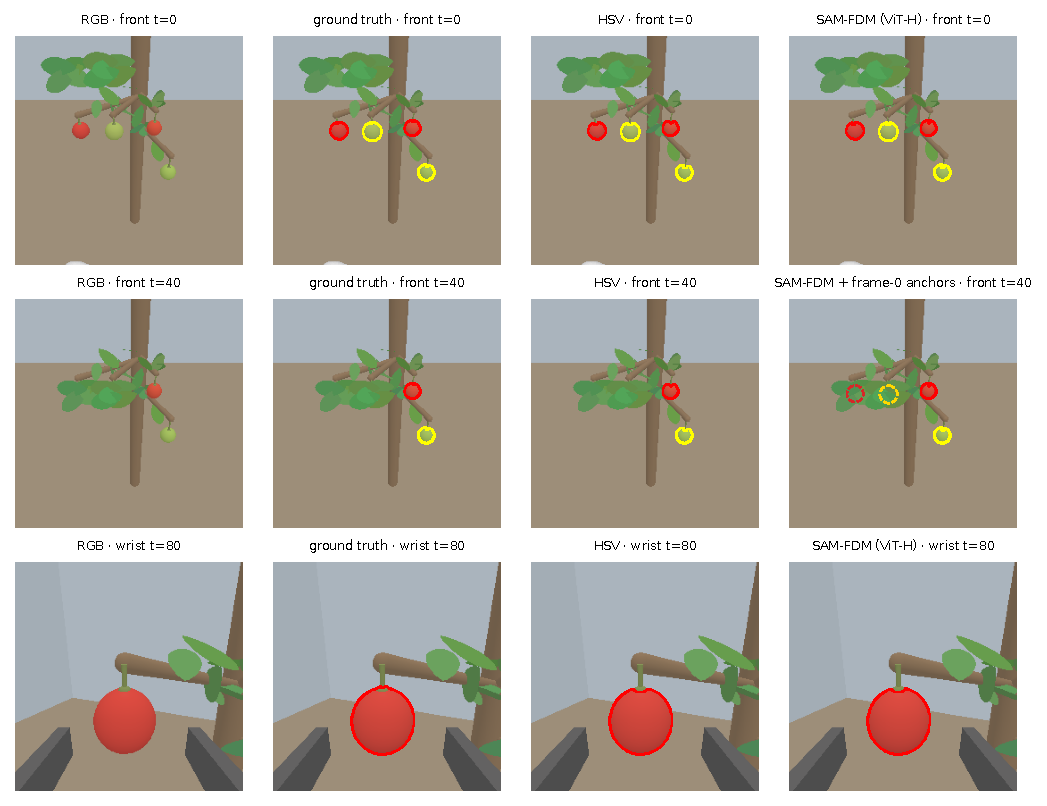
\includegraphics[width=0.74\linewidth]{fig8a_sam_qualitative}\\[2pt]
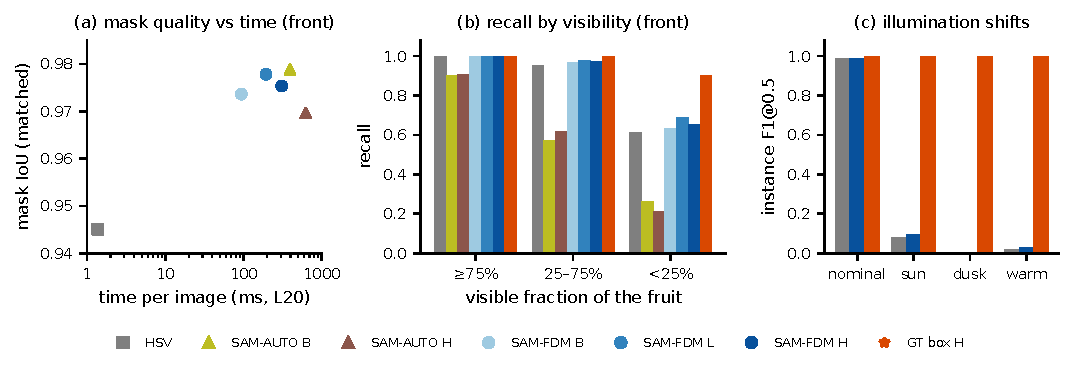
\includegraphics[width=\linewidth]{fig8b_sam_quantitative}
\caption{Fruit segmentation. Top: a FruitOccludedRipe validation episode before the gust (front, $t=0$), after it (front, $t=40$) and at contact (wrist, $t=80$); columns show the image, ground truth, HSV thresholds and \fdm\ (ViT-H), with red contours for ripe and yellow for unripe fruits. At $t=40$, dashed circles are the frame-0 anchors, which keep the two leaf-hidden fruits in memory. Bottom: (a) mask IoU versus latency; (b) front-camera recall by visible fraction; (c) F1 under illumination shifts.}
\label{fig:sam}
\end{figure}

\subsection{From RGB-D images to event memory (RQ6)}
\label{sec:res_chain}
Table~\ref{tab:chain} evaluates the complete chain on the 199 validation episodes using only the recorded front RGB-D frames, forward kinematics and the gripper state, with no simulator ground truth (per-task results with the K8 memory in Supplementary Table~S3).

\emph{Anchors, distances and events.} Frame-0 anchors recover 99.8\% of fruits with 99.5\% precision, a median localization error of 0.48~cm (90th percentile 0.58~cm), below a fifth of the fruit radius, and error-free ripeness; all 138 ripe fruits that the gust later hides have an anchor (Section~\ref{sec:res_anchor}). The perceived distance has a median near-range error of 0.34~cm (90th percentile 0.48~cm), well inside the accuracy specification above. Events detected from $\hat d_t$ match the ground truth exactly (F1 1.000, count exact in every episode, release error 0 frames), and the \pekm\ memories recover every ground-truth keyframe (Jaccard 0.948 for $k=4$, 0.941 for $k=8$, the differences being contact frames shifted by one or two frames). Consumer-grade depth noise leaves all results unchanged.

\emph{Grasp evidence closes the visual blind spot, and anchors beat per-frame detection.} With depth vacancy alone, the arm and the carried fruit occlude the anchor during carrying, so the release keyframe is late by a median of 16 frames and the memory Jaccard drops to 0.685; the nearly free gripper-holding cue removes the delay. Without anchors, the carried fruit is still detected as the nearest fruit: the release error grows to 52 frames and spurious events appear (precision 0.821, count exact in 62\% of episodes; 0.759 and 46\% in FruitCount), and even with hysteresis (precision 0.942) the memory Jaccard remains 0.421 (Fig.~\ref{fig:chain}).

\begin{table}[t]
\centering
\caption{Events and memory from perceived distances (199 validation episodes; plain detector, hysteresis in parentheses). Dist.\ err.: median / 90th-percentile error of $\hat d_t$ where $d_t \le 10$ cm. Rel.\ err.: median release-keyframe error (frames). Jaccard and KF recall: agreement of the K4 memory with the GT memory. For K8, Jaccard is 0.941 / 0.941 / 0.660 / 0.730 / 0.363 and KF recall 1.000 / 1.000 / 0.847 / 0.882 / 0.782 for the rows below GT.}
\label{tab:chain}
\footnotesize
\begin{adjustbox}{max width=\textwidth}\begin{tabular}{lcccccccc}
\toprule
Distance source & Dist.\ err.\ (cm) & P & R & F1 & Count & Rel.\ err. & Jaccard & KF recall\\
\midrule
GT (upper bound) & 0 / 0 & 1.000 & 1.000 & 1.000 & 1.00 & 0 & 1.000 & 1.000\\
\textbf{\fdm\ (ours)} & \textbf{0.34 / 0.48} & \textbf{1.000} & \textbf{1.000} & \textbf{1.000} & \textbf{1.00} & \textbf{0} & \textbf{0.948} & \textbf{1.000}\\
\fdm\ + depth noise & 0.31 / 0.46 & 1.000 & 1.000 & 1.000 & 1.00 & 0 & 0.948 & 1.000\\
Depth-only & 0.39 / 10.76 & 1.000 & 1.000 & 1.000 & 1.00 & 16 & 0.685 & 0.845\\
Post-gust anchors & 0.39 / -- & 1.000 & 0.743 & 0.853 & 0.50 & 0 & 0.741 & 0.880\\
Per-frame & 0.39 / 12.79 & 0.821 (0.942) & 1.000 & 0.902 (0.970) & 0.62 (0.85) & 52 & 0.421 & 0.755\\
\bottomrule
\end{tabular}\end{adjustbox}
\end{table}

\begin{figure}[t]
\centering
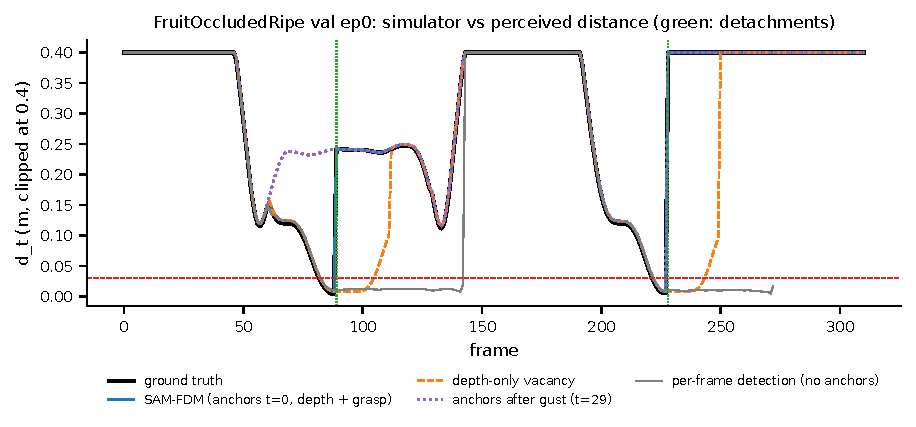
\includegraphics[width=0.82\linewidth]{fig_e6_perceived_distance}
\caption{Perceived versus ground-truth distance in one FruitOccludedRipe episode (vertical lines: detachments). \fdm\ follows the ground truth; depth-only vacancy confirms detachment late, post-gust anchors miss the hidden ripe fruit, and per-frame detection tracks the carried fruit.}
\label{fig:chain}
\end{figure}

\subsection{Spatial memory before occlusion is a precondition for event memory (RQ6)}
\label{sec:res_anchor}
The perception chain above builds its anchors at frame 0, before the wind gust. To isolate the role of this spatial memory, we rebuilt the anchors at frame 29, after the gust, with everything else unchanged, i.e.\ the same segmentation, depth, grasp evidence, detector and memory. Table~\ref{tab:anchors} and Fig.~\ref{fig:anchor} report the result per task.

\emph{Hidden ripe fruits disappear from memory.} In FruitOccludedRipe, post-gust anchors recover only 56.8\% of the fruits, against 99.6\% before the gust, and \emph{none} of the 138 ripe fruits that the leaves hide receives an anchor (0\% against 100\%). Over both tasks, this is the drop from 99.8\% to 78.3\% anchor recall. The anchors that are built are as good as before: precision 0.989 versus 0.994, localization error 0.49 versus 0.48~cm, ripeness error-free in both cases. The degradation therefore concerns \emph{when} the spatial memory is formed, not \emph{how accurately} it is measured.

\emph{The loss propagates to events and to the policy's memory.} Without an anchor, the robot's approach to a hidden ripe fruit produces no distance minimum. The median near-range distance error grows from 0.35 to 5.78~cm, and in more than a tenth of the near-range frames no fruit is perceived at all. Event recall falls from 1.000 to 0.450: 138 of the 251 picks go undetected, as many as there are leaf-hidden ripe fruits. Not a single FruitOccludedRipe episode keeps the correct pick count (0.00 versus 1.00). The K4 memory recovers only 73.1\% of its ground-truth keyframes (Jaccard 0.493 versus 0.948), so the frames reserved for picks would be spent on the wrong moments.

\emph{The failure is silent, and specific to occlusion.} Precision stays at 1.000 because every detected event is real, so a precision-based check would not reveal that half of the picks are missing. In FruitCount, where no fruit is hidden by foliage, frame-0 and frame-29 anchors give identical results in every metric, which confirms that the loss is caused by occlusion and not by the change of anchoring frame. Consumer-grade depth noise leaves the frame-0 results unchanged (localization error 0.45~cm). Remembering \emph{where} a fruit is, perceived while it was visible, is a precondition for remembering \emph{that} it was picked. In practice, a harvesting system should build its spatial memory when it first faces a plant, before its own motion, wind or leaf contact occlude the fruits, and keep that memory persistent.

\begin{table}[t]
\centering
\caption{Spatial memory before versus after occlusion (\fdm, ViT-H; 199 validation episodes; plain detector). Anchors are built at frame 0 (before the gust) or at frame 29 (after it); all other components are unchanged. Hidden ripe: leaf-hidden ripe fruits with an anchor. Dist.\ err.: median error of $\hat d_t$ where $d_t \le 10$ cm. Count: fraction of episodes with the exact pick count. Jaccard and KF recall: agreement of the K4 memory with the ground-truth memory.}
\label{tab:anchors}
\footnotesize
\setlength{\tabcolsep}{4pt}
\begin{adjustbox}{max width=\textwidth}\begin{tabular}{llcccccccccc}
\toprule
 & & \multicolumn{4}{c}{Spatial memory (anchors)} & & \multicolumn{3}{c}{Picking events} & \multicolumn{2}{c}{K4 memory}\\
\cmidrule(lr){3-6}\cmidrule(lr){8-10}\cmidrule(lr){11-12}
Task & Anchors at & Recall & Prec. & Loc.\ err.\ (cm) & Hidden ripe & Dist.\ err.\ (cm) & Recall & F1 & Count & Jaccard & KF recall\\
\midrule
FruitOccludedRipe & \textbf{frame 0 (ours)} & \textbf{0.996} & 0.994 & 0.48 & \textbf{138 / 138} & \textbf{0.35} & \textbf{1.000} & \textbf{1.000} & \textbf{1.00} & \textbf{0.948} & \textbf{1.000}\\
 & frame 0 + depth noise & 0.996 & 0.994 & 0.45 & 138 / 138 & 0.32 & 1.000 & 1.000 & 1.00 & 0.948 & 1.000\\
 & frame 29 & 0.568 & 0.989 & 0.49 & 0 / 138 & 5.78 & 0.450 & 0.621 & 0.00 & 0.493 & 0.731\\
\midrule
FruitCount & frame 0 (ours) & 1.000 & 0.996 & 0.48 & -- & 0.33 & 1.000 & 1.000 & 1.00 & 0.947 & 1.000\\
(control) & frame 29 & 1.000 & 0.996 & 0.48 & -- & 0.33 & 1.000 & 1.000 & 1.00 & 0.947 & 1.000\\
\midrule
Both tasks & frame 0 (ours) & \textbf{0.998} & 0.995 & 0.48 & \textbf{138 / 138} & 0.34 & \textbf{1.000} & \textbf{1.000} & \textbf{1.00} & 0.948 & 1.000\\
 & frame 29 & 0.783 & 0.993 & 0.49 & 0 / 138 & 0.39 & 0.743 & 0.853 & 0.50 & 0.741 & 0.880\\
\bottomrule
\end{tabular}\end{adjustbox}
\end{table}

\begin{figure}[t]
\centering
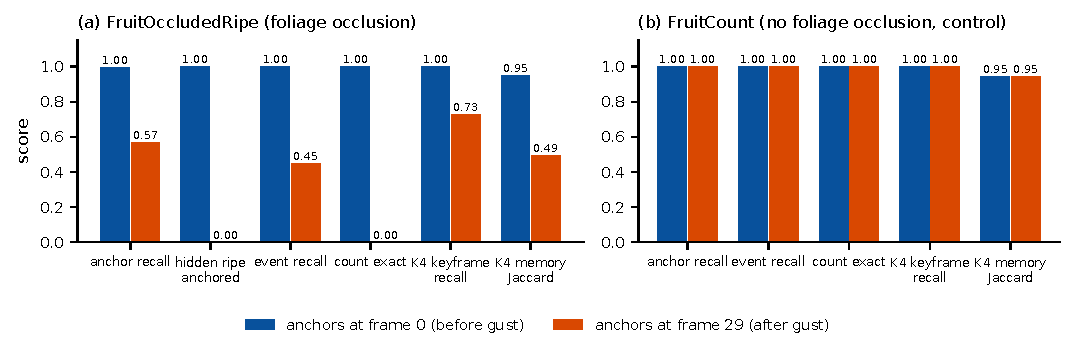
\includegraphics[width=\linewidth]{fig_anchor_timing}
\caption{How the timing of spatial memory propagates to event memory. Anchors built before the gust (frame 0, blue) or after it (frame 29, orange), with all other components unchanged. (a) In FruitOccludedRipe, post-gust anchoring loses every leaf-hidden ripe fruit, and the loss carries through to the detected picks, the pick count and the frames reserved in the K4 memory. (b) In FruitCount, without foliage occlusion, the two anchoring times are indistinguishable.}
\label{fig:anchor}
\end{figure}

\subsection{Closed-loop harvesting (RQ7)}
\label{sec:res_closed}
Table~\ref{tab:closed} reports closed-loop results on validation episodes 50--99 (150 trials per task and condition). \tbd{Main results after the sealed evaluation: success of K0/K4/K8 per task with paired differences, 95\% CIs and Holm-adjusted p-values; process metrics; stratification by quota $N$ (2 / 3 / 4--5); validity gates (engineering errors, complete blocks, per-decision frame audit).}

\begin{table}[t]
\centering
\caption{Closed-loop harvesting on validation episodes 50--99 (3 seeds; 150 trials per cell). Paired differences with 95\% bootstrap CIs; Holm-adjusted p-values over the primary family.}
\label{tab:closed}
\footnotesize
\begin{adjustbox}{max width=\textwidth}\begin{tabular}{llcccccc}
\toprule
Task & Memory & Success & Completion & Over-/wrong-pick & Drop & Steps & $\Delta$ vs K0 [95\% CI]\\
\midrule
FruitCount & K0 (uniform) & \tbd{} & \tbd{} & \tbd{} & \tbd{} & \tbd{} & --\\
 & K4 (PEKM) & \tbd{} & \tbd{} & \tbd{} & \tbd{} & \tbd{} & \tbd{}\\
 & K8 (PEKM) & \tbd{} & \tbd{} & \tbd{} & \tbd{} & \tbd{} & \tbd{}\\
FruitOccludedRipe & K0 (uniform) & \tbd{} & \tbd{} & \tbd{} & \tbd{} & \tbd{} & --\\
 & K4 (PEKM) & \tbd{} & \tbd{} & \tbd{} & \tbd{} & \tbd{} & \tbd{}\\
 & K8 (PEKM) & \tbd{} & \tbd{} & \tbd{} & \tbd{} & \tbd{} & \tbd{}\\
\bottomrule
\end{tabular}\end{adjustbox}
\end{table}

\subsection{Ablations and counterfactual controls (RQ7)}
\label{sec:res_ablation}
Table~\ref{tab:ablation} lists the test-time ablations of the K4 policy under the same paired protocol. \tbd{Ablation results: keyframe cap, radius, hard vs soft selection, signal source (GT, \fdm, noisy), counterfactual controls EVU/EVR/EVA, keyframe composition, training data.}

\begin{table}[t]
\centering
\caption{Ablations (test-time variants of the K4 policy unless noted; paired differences to the default configuration).}
\label{tab:ablation}
\footnotesize
\begin{adjustbox}{max width=\textwidth}\begin{tabular}{llcc}
\toprule
Factor & Setting & FruitCount $\Delta$ & FruitOccludedRipe $\Delta$\\
\midrule
Keyframe cap $k$ (trained) & 0 / 4 / 8 & \tbd{} & \tbd{}\\
Radius $r$ & 1 / 3 / 5 cm & \tbd{} & \tbd{}\\
Selection & hard (PEKM) / soft (PEKM-S, $\alpha=0.5$) & \tbd{} & \tbd{}\\
Signal source & GT / \fdm\ / GT + 1 cm noise & \tbd{} & \tbd{}\\
Counterfactual & EV / EVU / EVR / EVA & \tbd{} & \tbd{}\\
Keyframes & contact / release / both & \tbd{} & \tbd{}\\
Training data & clean (C0) / clean + DART-H (K0) & \tbd{} & \tbd{}\\
\bottomrule
\end{tabular}\end{adjustbox}
\end{table}

\subsection{Open-loop accuracy and closed-loop drift (RQ8)}
\label{sec:res_dart}
Table~\ref{tab:openloop} evaluates a uniform-memory policy trained on clean demonstrations in open loop, i.e.\ teacher-forced at the demonstrated states. Its median TCP errors are 1.7--2.4~cm at the end of a 16-step chunk and 0.7--1.1~cm near the fruit, an order of magnitude below the motion within a chunk, and it agrees with the demonstrated gripper direction in 98--99.5\% of decisions. Training and validation errors are nearly identical, so the policy generalizes to unseen layouts at the demonstrated states. In closed loop, however, small deviations accumulate into states that clean demonstrations do not cover, the covariate shift that DART-H targets; its perturbations (median 2.5~cm) match the scale of the open-loop errors. \tbd{Closed-loop C0 vs K0 comparison: success, harvest completion, failure modes.}

\begin{table}[t]
\centering
\caption{Open-loop (teacher-forced) accuracy of a uniform-memory policy trained on clean demonstrations (10 episodes per set). TCP error at horizons 1, 8 and 16 of the action chunk; near: horizon 16 while $d_t \le 10$ cm.}
\label{tab:openloop}
\footnotesize
\begin{adjustbox}{max width=\textwidth}\begin{tabular}{llccc}
\toprule
Set & Task & TCP error h1 / h8 / h16 (cm) & Near h16 (cm) & Gripper agreement\\
\midrule
Train & FruitCount & 0.44 / 1.23 / 1.83 & 0.75 & 99.5\%\\
Train & FruitOccludedRipe & 0.42 / 1.25 / 1.66 & 0.70 & 99.2\%\\
Validation & FruitCount & 0.51 / 1.37 / 2.38 & 1.14 & 98.0\%\\
Validation & FruitOccludedRipe & 0.40 / 1.32 / 1.75 & 0.78 & 98.9\%\\
\bottomrule
\end{tabular}\end{adjustbox}
\end{table}

\subsection{Memory content matters for VLA policies (supporting evidence)}
\label{sec:res_general}
The premise of this work, that the content of a fixed-budget memory influences a VLA policy, was verified on a general manipulation-memory benchmark (\tbd{cite RoboMME}) with the base policy, under sealed protocols with paired bootstrap and Holm adjustment (Table~\ref{tab:general}). Removing the history memory collapses success on a pattern-recall task from 66.7\% to 1.7\%, and halving the budget from 32 to 16 frames reduces it from 64.4\% to 26.7\%. Replacing a single memory slot changes the action loss with a slot-ranking reliability of 0.97--0.99 across four tasks: within a fixed budget, the choice of frames matters, which is exactly the decision that \pekm\ makes using the harvesting structure. \tbd{Generalization: success by quota $N$ and on unseen layouts from E7.}

\begin{table}[t]
\centering
\caption{Memory ablations of the base VLA on a general manipulation-memory benchmark (paired bootstrap, Holm-adjusted).}
\label{tab:general}
\footnotesize
\begin{adjustbox}{max width=\textwidth}\begin{tabular}{>{\raggedright\arraybackslash}p{4.8cm}>{\raggedright\arraybackslash}p{8.2cm}}
\toprule
Intervention & Result\\
\midrule
No history memory (pattern-recall task) & 66.7\% $\rightarrow$ 1.7\% ($-65.0$ pp, 95\% CI [$-81.7$, $-46.7$], $p<0.001$)\\
No memory (video-swap task) & $-11.7$ pp (95\% CI [$-20.0$, $-3.3$], $p=0.006$)\\
Budget 32 $\rightarrow$ 16 frames (pattern recall) & 64.4\% $\rightarrow$ 26.7\% ($-37.8$ pp, $p<0.001$)\\
Single-slot replacement (counterfactual action loss) & Slot-ranking reliability 0.97--0.99 over four tasks; cross-fitted relative gain 2.5--12.4\%\\
\bottomrule
\end{tabular}\end{adjustbox}
\end{table}

\subsection{Run-time cost (RQ8)}
\label{sec:res_cost}
At $t=1000$ frames, one \pekm\ selection takes 117~$\mu$s on a CPU core (39~$\mu$s for uniform sampling), negligible against one VLA inference (\tbd{VLA latency, ms}), and the memory footprint and inference cost of the policy are those of the uniform baseline, since the number of frames is unchanged. \fdm\ runs SAM once per episode (94 / 195 / 309~ms for ViT-B / L / H on one L20 GPU), and its per-frame work, projecting a few anchors and reading depth and gripper state, takes well under a millisecond. Detection itself is a threshold comparison per frame.

\section{Discussion}
\label{sec:discussion}

\subsection{From time-indexed to event-indexed memory}
The central lesson of this work is that the memory of an embodied agricultural agent should be organized around what happens, not around when it happens. The coverage analysis and its close agreement with measurement (Fig.~\ref{fig:theory}) show that the failure of uniform memory is structural. For any fixed budget, the fraction of interaction events that time-indexed memory retains vanishes as operation lengthens. This is precisely the regime of practical harvesting, in which a robot works continuously along a row rather than in short, isolated episodes. Enlarging the budget only postpones the problem, at a cost that grows quadratically. Event indexing removes the dependence on operating time altogether. Picks are short (about a dozen frames out of several hundred) but physically unambiguous: event detection is exact over a 1--4~cm plateau of the radius, set by fruit size rather than tuned. Reserving two slots per remembered pick makes the memory complete for the information the task needs (99.6\% of picks) at no cost in budget, latency or architecture.

The approach--act--leave structure is not specific to fruit picking. Pruning cuts, fruit thinning, flower pollination and spot spraying all consist of discrete interactions with plant organs. For each of them, the distance from the tool to the nearest organ still to be treated is an equally natural event signal, and the radius scales with organ size. We therefore expect event-centric memory to transfer to these operations with only a redefinition of the target set $\mathcal{P}_t$. It could serve as a general memory principle for agricultural manipulation, beyond the harvesting tasks studied here.

\subsection{Designing perception for memory}
The perception experiments yield two lessons for agricultural perception systems that feed a learned policy.

First, \emph{what perception must deliver is a specification, not a maximum}. Event-based memory tolerates up to about 1.5~cm of white noise or 2~cm of correlated noise in the distance signal, together with arbitrary independent dropouts and centimetre-level bias. \fdm\ is an order of magnitude more accurate than this specification (0.34~cm median error), and remains so under consumer-grade depth noise. This margin indicates that a cheaper detector or sensor can be substituted, and the scalar interface makes such substitution straightforward.

Second, \emph{memory starts with perception}. Leaf-hidden ripe fruits are recoverable only if they were anchored while visible: anchors built before the gust keep all 138 of them, anchors built after it none, and with them disappear 138 of the 251 picks and the correct count of every occluded-task episode (Section~\ref{sec:res_anchor}). The anchors themselves were equally accurate in both cases; what mattered was \emph{when} they were formed. Moreover, the failure is silent: every event that is still detected is correct, so precision-based monitoring would not reveal it. In practice this argues for a deliberate observation phase, or for anchoring fruits whenever they become visible during operation, as well as for redundant evidence of picking. The gripper-holding cue removed a 16-frame delay at essentially zero cost, so proprioceptive and tactile signals should be treated as perception inputs for event detection, not only as control feedback. Explicit anchors (geometric memory) and \pekm\ (visual memory of events) thus play complementary roles. Anchors remember \emph{where} fruits are, and the event memory lets the policy see \emph{what happened} to them.

\subsection{Compounding errors in end-to-end harvesting}
End-to-end policies are accurate in open loop: about 2~cm TCP error at the end of a chunk, and 98--99.5\% agreement on gripper actions. Accuracy at the demonstrated states, however, does not guarantee success in closed loop, where small deviations accumulate into states that clean demonstrations do not cover. For harvesting, where the gripper must enclose a 5-cm fruit, a few centimetres of drift is the difference between a grasp and a miss. Recovery data that covers this drift, generated without an expert in the loop and restricted to the phases where it is safe, addresses the data rather than the model. \tbd{Discussion of the closed-loop DART-H and PEKM results once available.}

\subsection{Practical implications}
For field robots, which run on embedded GPUs with tight memory and latency budgets, the budget efficiency of event memory matters directly. With \pekm, an 8-frame memory retains more pick information than a 16-frame uniform one, and a 16-frame memory more than a 32-frame one, at a selection cost of about 0.1~ms. Because the selection is a pure function of a logged scalar signal, every memory the policy saw can be reproduced and audited after the fact. This property is useful for diagnosing failures in the field and supports the transparency expected of autonomous agricultural machines.

\subsection{Towards memory-aware agricultural foundation models}
As vision--language--action and other foundation models enter agricultural robotics, the question of what such models remember will become as important as what they perceive. Agricultural tasks are long, repetitive and partially observable, and their success depends on a running account of the plants already treated, the fruits still hidden and the quota still open. HarvestMem shows that this account can be supplied without changing the model's architecture or adding parameters. A physically grounded event signal, a spatial memory of objects acquired while they are visible, and a parameter-free selection rule turn a generic memory-augmented policy into one that remembers what matters for the task. We view this decoupling as a practical path for adapting general-purpose robot foundation models to agriculture. The agricultural knowledge is encoded in \emph{what counts as an event}, which domain experts can specify and audit, rather than in additional network parameters.

\subsection{Limitations}
This study has several limitations.
\begin{itemize}
\item \textbf{Simulation.} The study is conducted in simulation. Fruits are rigid spheres; stems detach after a fixed holding time, and branch mechanics are simplified. Wind acts only during the observation phase, and fruits do not swing.
\item \textbf{Perception scope.} Colour prompts suffice for red and green fruits on a rendered canopy under the calibrated lighting, but fixed thresholds do not transfer to strongly different illumination (Table~\ref{tab:light}), even though SAM's masks do. Green fruits against green foliage, natural illumination and clustered fruits (e.g.\ tomato trusses or grapes) will require learned or illumination-normalized prompt generators, and an event definition for clusters.
\item \textbf{Robot and scene diversity.} One tree type and one arm were used for closed-loop evaluation, although the generator also supports a 6-DoF arm.
\item \textbf{Real-world validation.} Transfer to a real orchard has not been tested yet. A RealMan RM75-B with an EG2 gripper and an RGB-D camera, matching the simulated system, is the planned platform.
\item \textbf{Closed-loop scope.} \tbd{Add any limitation revealed by the closed-loop results.}
\end{itemize}

\subsection{Future work}
Several extensions follow directly from the framework:
\begin{enumerate}
\item The event detector already counts picks, and this count can be given to the policy as a short text prompt (e.g.\ ``picked 2 of 3''), giving an explicit symbolic memory alongside the visual one.
\item A lightweight learned memory manager could be trained from counterfactual action-loss signals and compared with the rule-based selection.
\item Anchors of hidden ripe fruits could guide active leaf pushing before the approach.
\item Wind can be extended to the whole episode with swinging fruits.
\item Sim-to-real transfer with domain randomization of illumination, fruit colour and foliage density.
\end{enumerate}

\section{Conclusions}
\label{sec:conclusions}

This paper showed that the time-indexed memory of current vision--language--action policies is structurally unsuited to selective harvesting, and proposed HarvestMem, which couples a spatial memory of 3D fruit anchors, acquired by promptable segmentation while fruits are visible, with an episodic memory that reserves the contact and detachment keyframes of picks in the policy's fixed memory budget. The main findings are:
\begin{enumerate}
\item Uniform memory covers completed picks as $c_U(t) \approx \min(1, (B-1)|S|/t)$ (to within 0.012); at 16 frames, coverage of the most recent pick falls from 97.8\% to 21.7\% after 600 frames.
\item Picking events are detected exactly from the end-effector-to-fruit distance over a 1--4~cm range of the radius, on clean and perturbed demonstrations alike.
\item Picking-Event Keyframe Memory retains 99.6\% of completed picks against 57.0\% for uniform memory, keeps the most recent pick at every decision time, and with 8 frames outperforms uniform memory with 16, at no additional cost.
\item From RGB-D images and proprioception, the SAM-based fruit distance module localizes fruits to 0.48~cm, recovers every leaf-hidden ripe fruit and reproduces the ground-truth events exactly.
\item Spatial memory acquired before occlusion is a precondition for event memory: anchors built after occlusion are just as accurate, yet they miss all 138 leaf-hidden ripe fruits (anchor recall 78.3\% versus 99.8\%), 138 of 251 picks in the occluded task go undetected, and no occluded-task episode is counted correctly.
\item Event memory tolerates 1.5--2~cm distance errors, dropouts and bias; prompted SAM gives the most accurate fruit masks, and its prompt generator is the component to adapt to field illumination.
\item \tbd{One sentence on closed-loop success with PEKM and DART-H (E7--E9).}
\end{enumerate}
By moving agricultural knowledge into the definition of events rather than into network parameters, HarvestMem offers a principled, auditable way to adapt robot foundation models to the long, partially observable operations of agriculture.


\section*{CRediT authorship contribution statement}
\tbd{Conceptualization, Methodology, Software, Validation, Formal analysis, Investigation, Data curation, Writing -- original draft, Writing -- review \& editing, Visualization, Supervision, Funding acquisition.}

\section*{Declaration of competing interest}
The authors declare that they have no known competing financial interests or personal relationships that could have appeared to influence the work reported in this paper.

\section*{Data availability}
Supplementary material (benchmark details, full radius sweep, further memory examples and per-task perception results) accompanies this article. The HarvestMem-Sim generator, demonstrations, sealed evaluation protocols (with SHA-256 digests), analysis scripts and raw per-episode results will be released at \tbd{repository URL} upon publication.

\section*{Acknowledgements}
\tbd{Funding sources and grant numbers.}

\bibliographystyle{elsarticle-harv}
\renewcommand{\bibfont}{\footnotesize}
\setlength{\bibsep}{0pt}
\bibliography{references}

\end{document}
